%==============================================================================
% Masters Thesis Document
% This document template is adapted by Lester James V. Miranda
% for his Masters thesis in Waseda University.
%
% Using LaTeX Template Version 2.5 (27/8/17)
% The template was downloaded from:
% http://www.LaTeXTemplates.com
%
% Version 2.x major modifications by:
% Vel (vel@latextemplates.com)
%
% This template is based on a template by:
% Steve Gunn (users.ecs.soton.ac.uk/srg/softwaretools/document/templates/)
% Sunil Patel (sunilpatel.co.uk/thesis-template/)
%
% This file is part of thesis-manuscript.
%
% thesis-mansucript is free software: you can redistribute it and/or modify
% it under the terms of the GNU General Public License as published by
% the Free Software Foundation, either version 3 of the License, or
% (at your option) any later version.
%
% thesis-manuscript is distributed in the hope that it will be useful,
% but WITHOUT ANY WARRANTY; without even the implied warranty of
% MERCHANTABILITY or FITNESS FOR A PARTICULAR PURPOSE.  See the
% GNU General Public License for more details.
%
% You should have received a copy of the GNU General Public License
% along with thesis-manuscript.  If not, see <http://www.gnu.org/licenses/>.
%
%==============================================================================

%------------------------------------------------------------------------------
%	PACKAGES AND OTHER DOCUMENT CONFIGURATIONS
%------------------------------------------------------------------------------

\documentclass[11pt,
            english,
            oneside,
            liststotoc,
            singlespacing,
            headsepline,
            consistentlayout]{style}
\usepackage[utf8]{inputenc}
%\usepackage[T1]{fontenc}
%\usepackage{mathptmx}
\usepackage[backend=biber,style=authoryear,natbib=true]{biblatex}
\usepackage[autostyle=true]{csquotes}
\usepackage{enumitem}
\usepackage{amsmath}
\usepackage{amssymb}
\usepackage{wrapfig}
\usepackage{algorithm}
\usepackage{algpseudocode}
\usepackage{threeparttable}
\usepackage{footmisc}
\usepackage{siunitx}
\usepackage{ntheorem}
\usepackage{mdframed}
\usepackage{array}
\usepackage{subcaption}

\addbibresource{bibliography.bib}

%------------------------------------------------------------------------------
%	DEFINITION
%------------------------------------------------------------------------------
\theoremstyle{definition}
\theoremheaderfont{\bfseries}
\newmdtheoremenv[
    leftmargin=40, rightmargin=20,
    backgroundcolor=gray!20, linecolor=gray!20,
    innertopmargin=10,
    ntheorem
]{definition}{Definition}[section]
%\newtheorem{definition}{Definition}[section]

%------------------------------------------------------------------------------
%   SIUNITX SETTINGS
%------------------------------------------------------------------------------
% set-up numbers
\sisetup{
    output-exponent-marker=\ensuremath{\mathrm{e}},
    round-mode=places, round-precision=2,
    separate-uncertainty=false,
    detect-weight=true,
    detect-family=true,
    detect-inline-weight=math
}
\newcommand{\hg}{\bfseries}

%------------------------------------------------------------------------------
%	OTHER SETTINGS
%------------------------------------------------------------------------------
\setcounter{tocdepth}{1}
\setitemize{itemsep=-0.2em}        % Modify spacing between items
%\renewcommand{\arraystretch}{1.2}  % Stretch tables

% Command for algorithm INPUT and OUTPUT
\algnewcommand\algorithmicinput{\textbf{Input:}}
\algnewcommand\INPUT{\item[\algorithmicinput]}
\algnewcommand\algorithmicoutput{\textbf{Output:}}
\algnewcommand\OUTPUT{\item[\algorithmicoutput]}

% Set-up footnotes
%\renewcommand{\thefootnote}{\fnsymbol{footnote}}

% Item settings
\setlist{parsep=0pt, listparindent=\parindent}

% Math fonts set-up
\DeclareMathAlphabet{\mathcal}{OMS}{cmsy}{m}{n}
\SetMathAlphabet{\mathcal}{bold}{OMS}{cmsy}{b}{n}
\newcommand{\bigO}{\mathcal{O}}
\newcommand\given[1][]{\:#1\vert\:}
%------------------------------------------------------------------------------
%	MARGIN SETTINGS
%------------------------------------------------------------------------------

\geometry{
    paper=letterpaper, % Change to letterpaper for US letter
    inner=2.5cm, % Inner margin
    outer=3.8cm, % Outer margin
    bindingoffset=.5cm, % Binding offset
    top=1.5cm, % Top margin
    bottom=1.5cm, % Bottom margin
    showcrop
}

%------------------------------------------------------------------------------
%	THESIS INFORMATION
%------------------------------------------------------------------------------

\thesistitle{
    Autoencoder-based Feature Extraction Techniques for Protein Function
    Prediction
}
\supervisor{Dr. Jinglu Hu}
\degree{Master of Engineering}
\author{Lester James V. Miranda}
\addresses{}

\subject{Masters Thesis of Lester James V. Miranda}
\keywords{
    machine learning,
    bioinformatics,
    feature extraction,
    multilabel classification
}
\university{Waseda University}
\department{Graduate School of Information, Production, and Systems}
\group{Furuzuki Neurocomputing Systems Laboratory}
\faculty{Information Architecture}

\AtBeginDocument{
\hypersetup{pdftitle=\ttitle}
\hypersetup{pdfauthor=\authorname}
\hypersetup{pdfcreator=\authorname}
\hypersetup{pdfproducer=\authorname}
\hypersetup{pdfkeywords=\keywordnames}
\hypersetup{pdfsubject=\subject}
}

\begin{document}

\frontmatter

\pagestyle{plain}

%------------------------------------------------------------------------------
%	TITLE PAGE
%------------------------------------------------------------------------------

\begin{titlepage}
\begin{center}
\vspace*{.02\textheight}
{\LARGE \bfseries \ttitle}\vspace{2.5cm} % Thesis title

{\Large 44161652-3: \authorname} % Author name
\vfill 

{\normalsize \degreename} \\[2.5cm] % Degree

{\normalsize Supervisor: \supname} \\[2.5cm] % Supervisor's name

{\normalsize \groupname} \\        % Laboratory affilation
{\normalsize \facname}   \\        % Faculty affiliation
{\normalsize \deptname}  \\[0.5cm] % Departmental affiliation

{\normalsize \univname} \\[0.5cm] % University affiliation

{\normalsize \today} % Current date
\end{center}
\end{titlepage}

%------------------------------------------------------------------------------
%	SECOND TITLE PAGE
%------------------------------------------------------------------------------
\begin{titlepage}
\begin{center}
\thispagestyle{empty}
\vspace*{.02\textheight}
{\ttitle} \\[2.5cm] % Thesis title
{44161652-3: \authorname} \\[2.5cm] % Author name
{
    A thesis submitted to the Graduate School of \\
    Information, Production, and Systems\\
    Waseda University\\
    in partial fulfillment of the requirements for the degree of
} \\[1.2cm]

{\degreename} \\[2.5cm]
{Supervisor: \supname} \vfill
{\deptname}\\[1.0cm]
{\univname}\\[1.0cm]
{\today} \vfill


\includegraphics[width=0.25\textwidth]{wasedaLogo}\\[0.1cm]
{Copyright \textcopyright 2018 44161652-3: \authorname} \\[0.2cm]
All Rights Reserved
\end{center}
\end{titlepage}


%------------------------------------------------------------------------------
%	ABSTRACT PAGE
%------------------------------------------------------------------------------

\begin{abstract}
\addchaptertocentry{\abstractname} % Add the abstract to the table of contents

%=============================================================================
% Abstract
% Copyright (c) 2018. Lester James V. Miranda
%
% This file is part of thesis-manuscript.
%
% thesis-mansucript is free software: you can redistribute it and/or modify
% it under the terms of the GNU General Public License as published by
% the Free Software Foundation, either version 3 of the License, or
% (at your option) any later version.
%
% thesis-manuscript is distributed in the hope that it will be useful,
% but WITHOUT ANY WARRANTY; without even the implied warranty of
% MERCHANTABILITY or FITNESS FOR A PARTICULAR PURPOSE.  See the
% GNU General Public License for more details.
%
% You should have received a copy of the GNU General Public License
% along with thesis-manuscript.  If not, see <http://www.gnu.org/licenses/>.
%
% Created by: Lester James V. Miranda <ljvmiranda@gmail.com>
%=============================================================================

\par Predicting protein functions is a fundamental task with applications in
medicine and healthcare. However, the cost and slow-pace of biochemical
techniques hinder this process, causing a major backlog to the number of
unannotated proteins we have today. Machine learning techniques are suitable to
this data-intensive task, but they require efficient representations of data.
Thus, it is important to ensure that our features are meaningful and relevant
to the classifier. 

\par In this work, we introduce two autoencoder-based techniques that extracts
task-relevant representations for better protein classification. We first
explored a stacked denoising autoencoder, commonly-used in images, and examined
its efficacy in the protein domain. Then, we designed an autoencoder
architecture that extracts task-relevant features by letting the neurons
compete mutually with one another. The features derived by these autoencoders
are fed to a binary-relevance support-vector machine for classification.  We
tested both models on two protein benchmarks, investigating the effects of each
hyperparameter and measuring model quality, then we compared its performance
against other techniques in literature.

\par Results show that our proposed models perform better than other methods,
suggesting that extracting \emph{relevant} features, not mere feature
extraction, is crucial. Moreover, both models outperformed the baseline, i.e. a
model without feature extraction, indicating that it is important to derive
new features than using a protein's raw attributes.  Lastly, the
mutually-competitive autoencoder outperforms SdAE\textemdash exhibiting not
only a finer control during extraction, but improved classifier performance.
Overall, our work demonstrated the benefit of using these autoencoder-based
methods to extract task-relevant features for better protein classification.


\vfill
\noindent \textbf{Keywords}\textemdash\keywordnames
\end{abstract}

%------------------------------------------------------------------------------
%	ACKNOWLEDGEMENTS
%------------------------------------------------------------------------------

\begin{acknowledgements}
\addchaptertocentry{\acknowledgementname} % Add the acknowledgements to the table of contents

\end{acknowledgements}

%------------------------------------------------------------------------------
%	LIST OF CONTENTS/FIGURES/TABLES PAGES
%------------------------------------------------------------------------------

{
\hypersetup{linkcolor=black}
\tableofcontents % Prints the main table of contents
\listoffigures % Prints the list of figures
\listoftables % Prints the list of tables
}
%------------------------------------------------------------------------------
%	SYMBOLS
%------------------------------------------------------------------------------

\begin{symbols}{ll} % Include a list of Symbols (a three column table)

% dimensions
$N$                         & number of samples         \\
$q$                         & number of labels          \\
$d$                         & number of features        \\

\addlinespace % data
$x$                         & raw feature              \\
$x^{\prime}$                & extracted feature        \\
$\widetilde{x}$             & corrupted feature        \\
$\widehat{x}$               & reconstructed feature    \\
$y$                         & ground-truth label       \\
$\widehat{y}$               & prediction               \\


\addlinespace % functions
$f$                         & encoder function          \\
$g$                         & decoder function          \\
$L$                         & loss function             \\
$q^{\prime}$                & corrupting function       \\
$h$                         & classifier                \\

\addlinespace % learnable parameters 
$\theta$                    & network weight parameters \\
$W$                         & classifier parameters     \\

\addlinespace % hyperparameter
$k$                         & percentage of winners to keep \\
$\alpha$                    & competition parameter         \\
$e$                         & encoding dimension            \\

\end{symbols}


%------------------------------------------------------------------------------
%	THESIS CONTENT - CHAPTERS
%------------------------------------------------------------------------------

\mainmatter % Begin numeric (1,2,3...) page numbering

\pagestyle{thesis} % Return the page headers back to the "thesis" style

%=============================================================================
% Introduction
% Copyright (c) 2018. Lester James V. Miranda
%
% This file is part of thesis-manuscript.
%
% thesis-mansucript is free software: you can redistribute it and/or modify
% it under the terms of the GNU General Public License as published by
% the Free Software Foundation, either version 3 of the License, or
% (at your option) any later version.
%
% thesis-manuscript is distributed in the hope that it will be useful,
% but WITHOUT ANY WARRANTY; without even the implied warranty of
% MERCHANTABILITY or FITNESS FOR A PARTICULAR PURPOSE.  See the
% GNU General Public License for more details.
%
% You should have received a copy of the GNU General Public License
% along with thesis-manuscript.  If not, see <http://www.gnu.org/licenses/>.
%
% Created by: Lester James V. Miranda <ljvmiranda@gmail.com>
%=============================================================================

\chapter{Introduction}
\label{Introduction}

\par In bioinformatics, predicting a protein's function is a fundamental
task. Once accomplished, we can use our knowledge of protein functions to
various applications such as drug-design or disease identification
(\cite{baldi2001bioinformatics}). However, acquiring this information is
difficult due to the slow and expensive nature of existing biochemical
techniques today (\cite{cozzetto2017computational}). As the number
of proteins discovered by high-throughput methods increases,
the backlog of unannotated protein data piles up (\cite{gaudet2017gene}). This
then calls for a fast, accurate, and efficient set of prediction techniques
in the face of ``genomic big data.''
  
\par Machine learning has shown promise in complex tasks involving large
amounts of data (\cite{chen2014data}). They have been exceptional in
recognizing patterns and learning from a vast number of examples
(\cite{lecun2015deep}). Before prediction, a machine learning model must
discern a pattern from a dataset, and use it to infer the category, or
\textit{class}, a new sample belongs to. Because most proteins can perform
multiple functions at once, we frame the protein function prediction problem
as a multilabel classification task. In this manner, the primary question
becomes:

\begin{quote}
    \itshape
    \small
    Given a set of protein characteristics, what can we infer about
    its function/s?
\end{quote}

\noindent It is important to note that the effectiveness of a classification
model strongly depends on the pattern it learns, and how well it represents
the input data provided.

\par Feature extraction aims to represent raw data into a form beneficial to
a machine learning model. Although it is entirely possible to manually
engineer characteristics, or \textit{features}, from a dataset, it is
labor-intensive and requires thorough domain-expertise
(\cite{bengio2013representation}). Instead, it is preferable to automatically
derive useful information from our inputs and ensure that the new features
are relevant. The better a feature extraction method can represent raw data,
the easier a classification model can discriminate between its samples. For
protein datasets, extracting \textit{relevant} information is challenging for
two reasons: protein samples are (1) noisy, and (2) high-dimensional. Noise,
inherent in data-acquisition and intrinsic to biological complexity,
introduces irrelevant information to the classification task. On the other
hand, high-dimensional datasets suffer from the \textit{curse of
dimensionality}, further complicating the discrimination process.
Distinguishing which characteristics are important and transforming them into
features useful to a predictor is essential in identifying protein functions.

\newpage

\par This work's overarching theme is on the effect of \textit{extracting
relevant features} on the performance of a multilabel classification model in
predicting protein functions. We put emphasis on feature relevance, given the
noisy and high-dimensional nature of protein data. We hypothesize that by
obtaining relevant features, we can achieve higher classification performance
than naively extracting features or not extracting them at all. The models
that we will introduce in this work were based from an autoencoder neural
network. For the time being, know that autoencoders learn new representations
by actively reconstructing the input with the presence of information
bottlenecks. We studied two autoencoder architectures, and tested them on
protein benchmarks. The main contributions of this research are as follows:

\begin{itemize}
    \item We applied a stacked denoising autoencoder, a technique
    commonly-used in image denoising, to the protein function prediction problem.
    \begin{quote}
    \par We have demonstrated the efficacy of the autoencoder in a different
    problem domain by learning \textit{robust} features to aid multilabel
    classification. However, autoencoder training is inherently greedy, and
    motivating the network to learn sparse yet relevant features should
    offset this problem.
    \end{quote}
    \item We designed a mutually-competitive autoencoder architecture that
    motivates the creation of sparse yet relevant features from raw data.
    \begin{quote}
    \par We have proven that by learning \textit{relevant} representations
    of the raw inputs, classification performance can improve. This architecture
    outperformed not only a model without feature extraction, but also other
    feature extraction methods by a significant margin. 
    \end{quote}
\end{itemize}



\par \noindent This document is divided into five (5) chapters, with the rest
organized as follows:

\begin{itemize}
    \item \textsc{Chapter \ref{BackgroundChapter}} \textit{(Background of the
    Study)} provides an overview of the protein function prediction problem,
    the idea behind feature extraction, and the formulation of a multilabel
    classification problem. It also reviews related works that will be
    benchmarked against our proposed method.
    \item \textsc{Chapter \ref{SDAEChapter}} \textit{(Feature Extraction
    using a Stacked Denoising Autoencoder for Protein Function Prediction)}
    investigates the use of denoising autoencoders in the protein function
    prediction problem in a multilabel setting.
    \item \textsc{Chapter \ref{SelectiveChapter}} \textit{(Selective Feature
    Extraction using a Mutually-Competitive Autoencoder)} describes our proposed
    autoencoder architecture and key experiments that examine its performance
    on a protein function prediction task.
    \item \textsc{Chapter \ref{ConclusionsChapter}} \textit{(Conclusions)} gives
    a concise summary of this research, key insights, and potential avenues for
    future research.
\end{itemize}
%=============================================================================
% Background
% Copyright (c) 2018. Lester James V. Miranda
%
% This file is part of thesis-manuscript.
%
% thesis-mansucript is free software: you can redistribute it and/or modify
% it under the terms of the GNU General Public License as published by
% the Free Software Foundation, either version 3 of the License, or
% (at your option) any later version.
%
% thesis-manuscript is distributed in the hope that it will be useful,
% but WITHOUT ANY WARRANTY; without even the implied warranty of
% MERCHANTABILITY or FITNESS FOR A PARTICULAR PURPOSE.  See the
% GNU General Public License for more details.
%
% You should have received a copy of the GNU General Public License
% along with thesis-manuscript.  If not, see <http://www.gnu.org/licenses/>.
%
% Created by: Lester James V. Miranda <ljvmiranda@gmail.com>
%=============================================================================

\chapter{Background of the Study}
\label{BackgroundChapter}

\par In this chapter, we begin by looking into the problem of protein
function prediction in the lens of how protein data is usually represented
(Sec. \ref{ProteinFunctionPrediction}). Then, armed with the knowledge that
proteins can perform multiple functions at once, we will frame the protein
function prediction problem as a multilabel classification task (Sec.
\ref{MultilabelClassification}). We will argue that learning new
representations from data is vital to accomplish this task (Sec.
\ref{FeatureExtraction}), and at the same time introduce the autoencoder
neural network as basis for our methods. We then examine
previous works that have tackled this problem with a similar approach (Sec.
\ref{LiteratureReview}) and finally, express our research motivation
(Sec. \ref{Motivation}) and formulate research questions and hypotheses
throughout this work.


\section{Protein Data Representation}
\label{ProteinFunctionPrediction}

Approaching the protein function prediction problem requires an
understanding of how protein data is often represented. We always
describe proteins in two ways: first by their (1) \textit{features} or
characteristics, and then by their (2) \textit{labels} or functional
categories.

\subsection{Protein features from high-throughput methods}

\par High-throughput sequencing techniques ushered in the emergence of
genomic big data (\cite{reuter2015high}). Scientists conducted various
experiments (e.g. DNA microarray, phylogenetic trees, etc.) to profile
protein sequences, resulting to huge amounts of structured data available for
use. These datasets facilitated protein function prediction, be it through
biochemical or computational means (\cite{eisenberg2000protein,
marcotte1999combined}). Similarly, this work will use two protein benchmarks,
Yeast and Genbase, derived from these experiments.

\par We define a \textit{protein feature set} as a matrix $\mathbf{X}$ where
each row and column is represented as a protein sample $i=1\dots N$ and a
specific measurement $j=1\dots d$ respectively. Both Yeast and Genbase
datasets were formed from microarray gene expression data, with the former
containing phylogenetic profiles as additional information. Succintly, the
raw feature set is defined as $\mathbf{X} \in \mathbb{R}^{N \times d}$ where $N$
is the number of protein samples and $d$ is the dimension or number of
attributes.

\par It is vital to spend some time emphasizing that noise is intrinsic to
high-throughput data (\cite{hong2013estimating}). A DNA microarray, for
example, is formed by probing unique regions of a gene in order to detect
expressions present in the tissue. Probing is sometimes conducted
heterogeneously, for ``different parts of the body, different [organisms], or
different phases of the cellular cycle'' (\cite{nguyen2009noise}). Each step
has the potential to introduce noise that may be detrimental to our task. To
a greater extent, extracting features from noisy data can compound its effect
and damage our classification model. Later on, we will discuss the denoising
autoencoder as a way to reduce the effect of noise from our raw features; but
first, let's look into what these features correspond to\textemdash a
protein's function.

\subsection{Protein functions}

\par Proteins perform a variety of functions to maintain our survival. They
can be seen in almost every facet of our biological processes: cell
reproduction, signalling, metabolism, and etc. By design, a singular protein
can perform multiple functions at once. This means that there is a
one-to-many relationship between protein samples and its function/s. A good
example is the YAL041W protein found in \textit{S. cerevisiae} or baker's
yeast (\cite{elisseeff2001kernel}) in Figure \ref{demo:yeast_go}. 


\begin{figure}[!h]
  \centering
  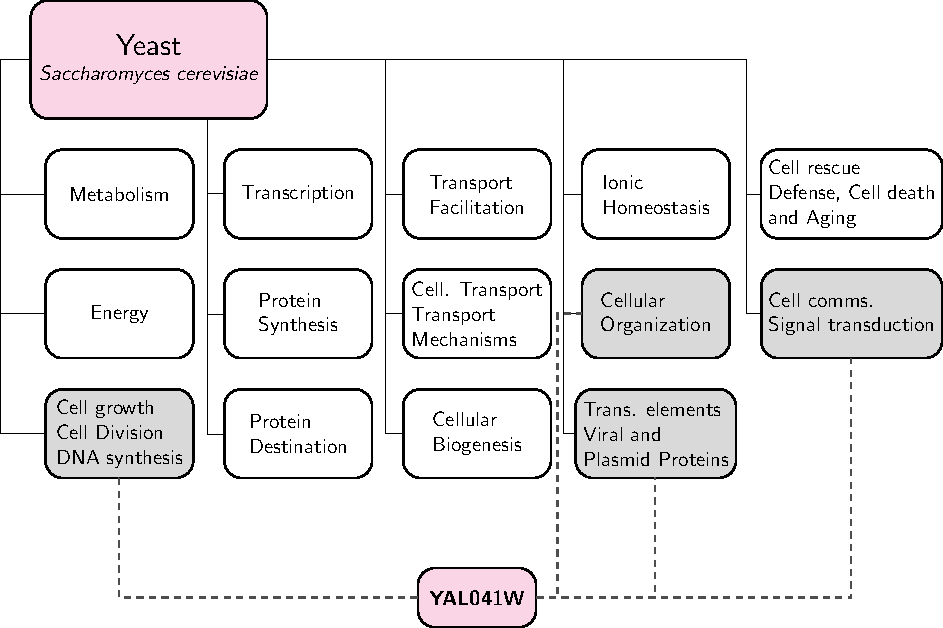
\includegraphics[width=0.75\textwidth]{ch01/demo_ontology}
  \caption{Functional categories of protein YAL041W in \textit{S. cerevisiae}}
  \label{demo:yeast_go}
\end{figure}

\noindent YAL041W is associated with multiple functional categories: cell growth,
organization, communication, and viral detection. To an extent, these
categories are not related to one another yet they are wilfully performed by
a single protein.

\par We define a set of protein functions or \textit{labels} as a binary
matrix $\mathbf{Y}$ where each row $i=1 \dots N$ is a protein sample, and
each column $j=1 \dots q$ is a protein function (designated as $\lambda$).
The size of $q$ depends on the number of possible labels in the dataset. In
addition, a protein labelset (a row vector) $\mathbf{y}_n$ is encoded as a
one-hot vector of size $q$. Say we're given a protein sample $n$ that performs
functions $\lambda_1, \lambda_4,$ and $\lambda_5$ in a set that only has
five functional categories, $q=5$, then we express its labelset as:

\[
    \mathbf{y}_n = \left[\begin{matrix}
        1 & 0 & 0 & 1 & 1
    \end{matrix} \right]
\]

More formally, we represent a set of protein labelsets as $\mathbf{Y} \in
\{0,1\}^{N \times q}$, where each row-vector $\mathbf{y}_n \in \{0,1\}^q$
is a labelset containing $q$ labels $\lambda$. 


\newpage
Together, we have the following definition:

\begin{definition}{}
A protein dataset $\mathcal{D}$ consists of $N$ pairs of feature and label
vectors $\{(\mathbf{x}_i, \mathbf{y}_i)\}_{i=1}^{N}$ where $\mathbf{x}_i \in
\mathbb{R}^d$ and $\mathbf{y}_i \in \{0,1\}^q$. In matrix-form, $\mathcal{D}$
consists of feature and label matrices, $\mathcal{D} = \langle \mathbf{X},
\mathbf{Y} \rangle$ where $\mathbf{X} \in \mathbb{R}^{N \times d}$ and
$\mathbf{Y} \in \{0,1\}^{N \times q}$.
\end{definition}

\par We will use this definition as we formulate the protein function
prediction problem as a multilabel classification task.


\section[Protein Function Prediction as a Multilabel Classification Task]
{Protein Function Prediction as a Multilabel\\Classification  (MLC) Task}
\label{MultilabelClassification}

\par Classification is one of the most common tasks in machine learning
(\cite{herrera2016multilabel}). Given input features $\mathbf{X}$ and its
label $y$, the goal is to find a mapping function $\mathcal{H}: \mathbf{X}
\rightarrow y$ that can accurately associate each set of attributes to its
particular label. For prediction, we then use the mapping function as
$\mathcal{H}: \mathbf{X} \rightarrow \widehat{y}$. A good example is image
classification, where given an image, the classifier must be able to
distinguish what particular object (or animal) it belongs to.

\begin{figure}[!h]
  \centering
  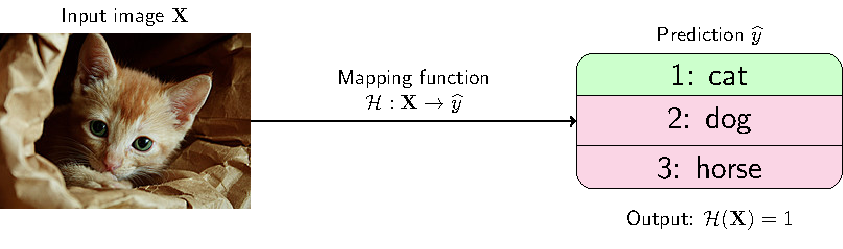
\includegraphics[width=0.70\textwidth]{ch01/demo_tradclass}
  \caption[Demonstration of traditional classification in images]
  {Demonstration of traditional classification in images.\\Cat photo
  from ImageNet (\cite{russakovsky2015imagenet})}
  \label{demo:traditional}
\end{figure}

\par However, proteins can perform multiple functions at once, and the
traditional definition of classification does not apply to the given task.
Instead, the goal is to discriminate between \textit{multiple labels} and
associate them to the feature set. An apt counterpart to image classification
is scene classification (\cite{boutell2004learning}), where multiple objects
(or animals) are associated to a given image.

\begin{figure}[!h]
  \centering
  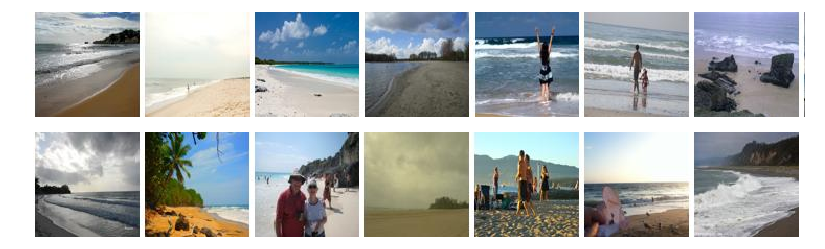
\includegraphics[width=0.95\textwidth]{ch01/demo_multilabel}
  \caption[Demonstration of multilabel classification]
  {Demonstration of multilabel classification.\\Beach photo
  from ImageNet (\cite{russakovsky2015imagenet})}
  \label{demo:multilabel}
\end{figure}

\newpage
\par Protein function prediction behaves similarly to scene classification:
given a protein sample (i.e., the image/scene), we are required to find the
functional categories associated with it (i.e., the objects in the scene).
This task is known as \textit{multilabel classification} (MLC). Notice that
in MLC, for each label $\lambda$, we only have two classes: $0$ (does not
belong to $\lambda$) and $1$ (belongs to $\lambda$). Thus, MLC is akin to
doing binary classification for each label. Formally, we define the multilabel
classification task as:

\begin{definition}{}
Given a dataset $\mathcal{D}$, find a function $\mathcal{H}$ that maps the
feature matrix $\mathbf{X}$ to a set of labels $\mathbf{Y}$, i.e.,
$\mathcal{H}: \mathbf{X} \rightarrow \mathbf{Y}$. For any unseen instance
$\mathbf{x} \in \mathcal{X}$, where $\mathcal{X} \in \mathbb{R}^d$, we
predict its corresponding label vector $\mathbf{\widehat{y}}$ via
$\mathcal{H}(\mathbf{X}) \subseteq \mathcal{Y}$ where $\mathcal{Y} = \{y_1,
y_2, \dots, y_n, \dots, y_q\}$ and $y_n \in \{0,1\}$\footnote{Adapted from
\cite{zhang2014review}}.
\end{definition}

\par Next, we will discuss a commonly-used approach in solving multilabel
classification problems: binary relevance.

\subsection{Binary relevance in multilabel classification}

\par Binary relevance (BR) decomposes a multilabel problem into a series of
single-label classification tasks (\cite{godbole2004discriminative,
tsoumakas2007multilabel}). The concept is to take any ``off-the-shelf''
classifier $h$ and train it on each label $\lambda$, fitting a total of $q$
classifiers as seen in Figure \ref{demo:binaryrelevance}. Further
modifications to BR include combining labels, or building chains of
classifiers (\cite{read2009classifier}). However, due to BR's conceptual
simplicity and time-complexity\footnote[2]{
    Most problem-transformation techniques have an overhead time-complexity
    depending on the classifier $h$. For Binary relevance, we have $\bigO(q
    \cdot h(N, d))$. At inference, the complexity is $\bigO(q
    \cdot h(d))$. This is relatively faster compared to Classifier Chains
    $\bigO(q \cdot h(N, d + q))$ or Label Ranking $\bigO(q^{2} \cdot h(N, d))$
    (\cite{zhang2014review}).
}, it has been widely used in literature (\cite{zhang2017binary}).

\begin{figure}[!h]
  \centering
  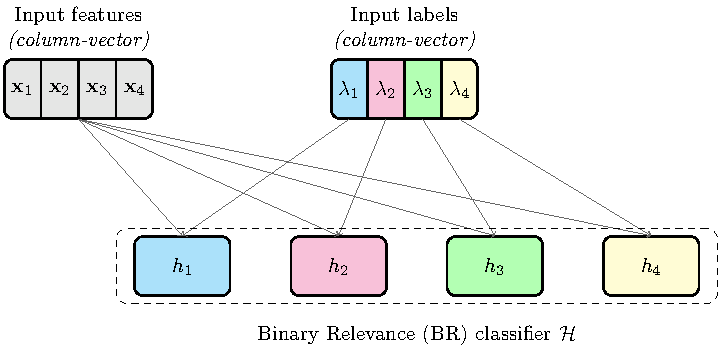
\includegraphics[width=0.65\textwidth]{ch01/demo_binaryrelevance}
  \caption[Binary relevance classification diagram]
  {Binary relevance classification diagram.\\Train $q$ classifiers $h$ for each
  label $\lambda$}
  \label{demo:binaryrelevance}
\end{figure}

\par BR falls under one of the two main approaches in classifying multilabel data:
problem transformation and algorithm adaptation. The former, where BR
belongs, transforms the multilabel problem into separate single-label binary
classification tasks while the latter adapts a classifier to directly handle
multilabel data (\cite{tsoumakas2007multilabel}).

\par We focus on BR for it is easier to treat the classifier as a separate
module from the feature extractor, and it is a simple yet effective method
for multilabel classification (\cite{luaces2012binary}). With BR, a
classifier can be decoupled from a feature extractor, enabling the former to
be tested on variants of the latter. Another reason is that the literature on
problem transformation techniques is extensive enough to enable benchmarking
of different multilabel classifiers in the future (\cite{zhang2014review,
madjarov2012extensive}).

\par This research will concentrate on finding good representations for the
BR classifier to solve the problem of protein function prediction. The
process of obtaining new features from raw data is called \textit{feature
extraction}, and is one of the core ideas in this work. Even if a BR
classifier can stand on its own, we hypothesize that higher performance can
be achieved with the extracted features than the raw data itself.

\section{Extracting Features for Better Data Representation}
\label{FeatureExtraction}

\par One of the core ideas in this work is feature extraction\footnote{
  Feature extraction has been referred to in various ways in literature:
  feature learning, representation learning, manifold learning, etc. We will
  use the term ``feature extraction'' in this work.
}\textemdash where new features are derived from raw attributes for better
data representation, and consequently, better classification. The success of
machine learning algorithms depends on data representations, for it can
entangle manifolds or explanatory factors of variation behind the data
(\cite{bengio2013representation}). 

\par More formally, the goal is to learn a mapping $\phi$ such that $\phi:
\mathbf{X} \rightarrow \mathbf{X}^{\prime}$, where $\mathbf{X}^{\prime}$
represents the extracted features useful\footnote{
  We will preemptively state that ensuring a feature set is useful will
  be the prime motivation of this work. We will attempt to define ``usefulness''
  or \textit{relevance} in Sec. \ref{Motivation}
} to a classifier $\mathcal{H}$. We
hypothesize that using $\mathbf{X}^{\prime}$ should provide better
classification (perhaps measured in accuracy, F-score, etc.) than just using
the raw attributes $\mathbf{X}$. The proceeding section will give a
simple demonstration using the XOR gate to illustrate this idea.

\subsection{A simple demonstration using the XOR gate}

\par Creating new features can be best illustrated with the XOR gate. The
goal is to separate binary 0's and 1's of the gate output. We take two
inputs $\mathbf{x} = \langle x_{1}$, $x_{2} \rangle, x_1, x_2 \in \{0,1\}$ as
features and its output $y_{i} \in \{0,1\}$ as the label. With $N=4$ samples
representing all possible bit-combinations, a dataset
$\mathcal{D}=\{(\mathbf{x}_{i}, y_{i})\}_{i=1}^{4}$ can be constructed as:

\[
    \mathcal{D} = \{(0,0,0), (0,1,1), (1,0,1), (1,1,0)\}
\]

Assuming we only have access to a linear classifier, the feature-space shown
in Figure \ref{demo:xor} (\textit{left}) proves that classifying the samples
is difficult due to its linear inseparability\textemdash that is, drawing a
single line to perfectly separate the X's and O's is impossible.
However, if a new feature-space $\mathbf{x}^{\prime}$ is engineered in such a
way that $\mathbf{x}^{\prime} = \langle {x}^{\prime}_{1}, {x}^{\prime}_2 \rangle$ where 
$x^{\prime}_{1} = \text{AND}(\bar{x}_{1}, x_{2})$ and $x^{\prime}_{2}
= \text{AND}(x_{1}, \bar{x}_{2})$, then it is possible to transform $\mathcal{D}$
into dataset $\mathcal{D}^{\prime}=\{(\mathbf{x}^{\prime}_{i}, y_{i})\}_{i=1}^{4}$
where:

\[
    \mathcal{D}^{\prime} = \{(0,0,0), (1,0,1), (0,1,1), (0,0,0)\}
\]

\par It can then be seen from Figure \ref{demo:xor} (\textit{right}) that
$\mathcal{D}^{\prime}$ is now a linearly separable problem. In this
demonstration, it is evident that hand-engineering features, or
\textit{extracting new features} has been helpful. However, with large
datasets, it will be tedious to manually find useful representations from
data. It is much preferable to automate the whole process. In the next
section, we will turn our attention to an effective way of learning $\phi$ in
a parameterized fashion\textemdash the autoencoder neural network.

\begin{figure}[!t]
  \centering
  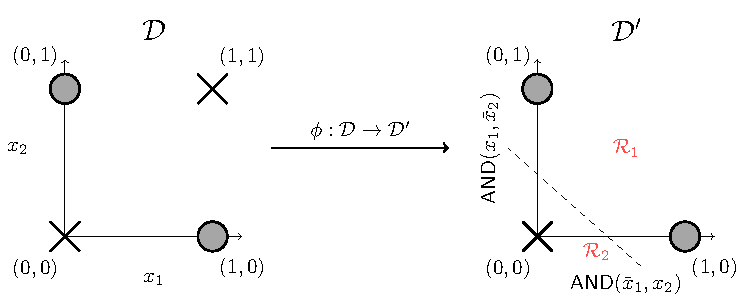
\includegraphics[width=0.75\textwidth]{ch01/demo_xor}
  \caption[Illustration of feature extraction using the XOR gate]
    {Illustration of feature extraction using the XOR gate.\\ Binary `1's are
    represented as circles while binary `0's as cross-marks.}
  \label{demo:xor}
\end{figure}

\subsection{The autoencoder neural network}

\begin{wrapfigure}{r}{0.5\textwidth}
  \centering
  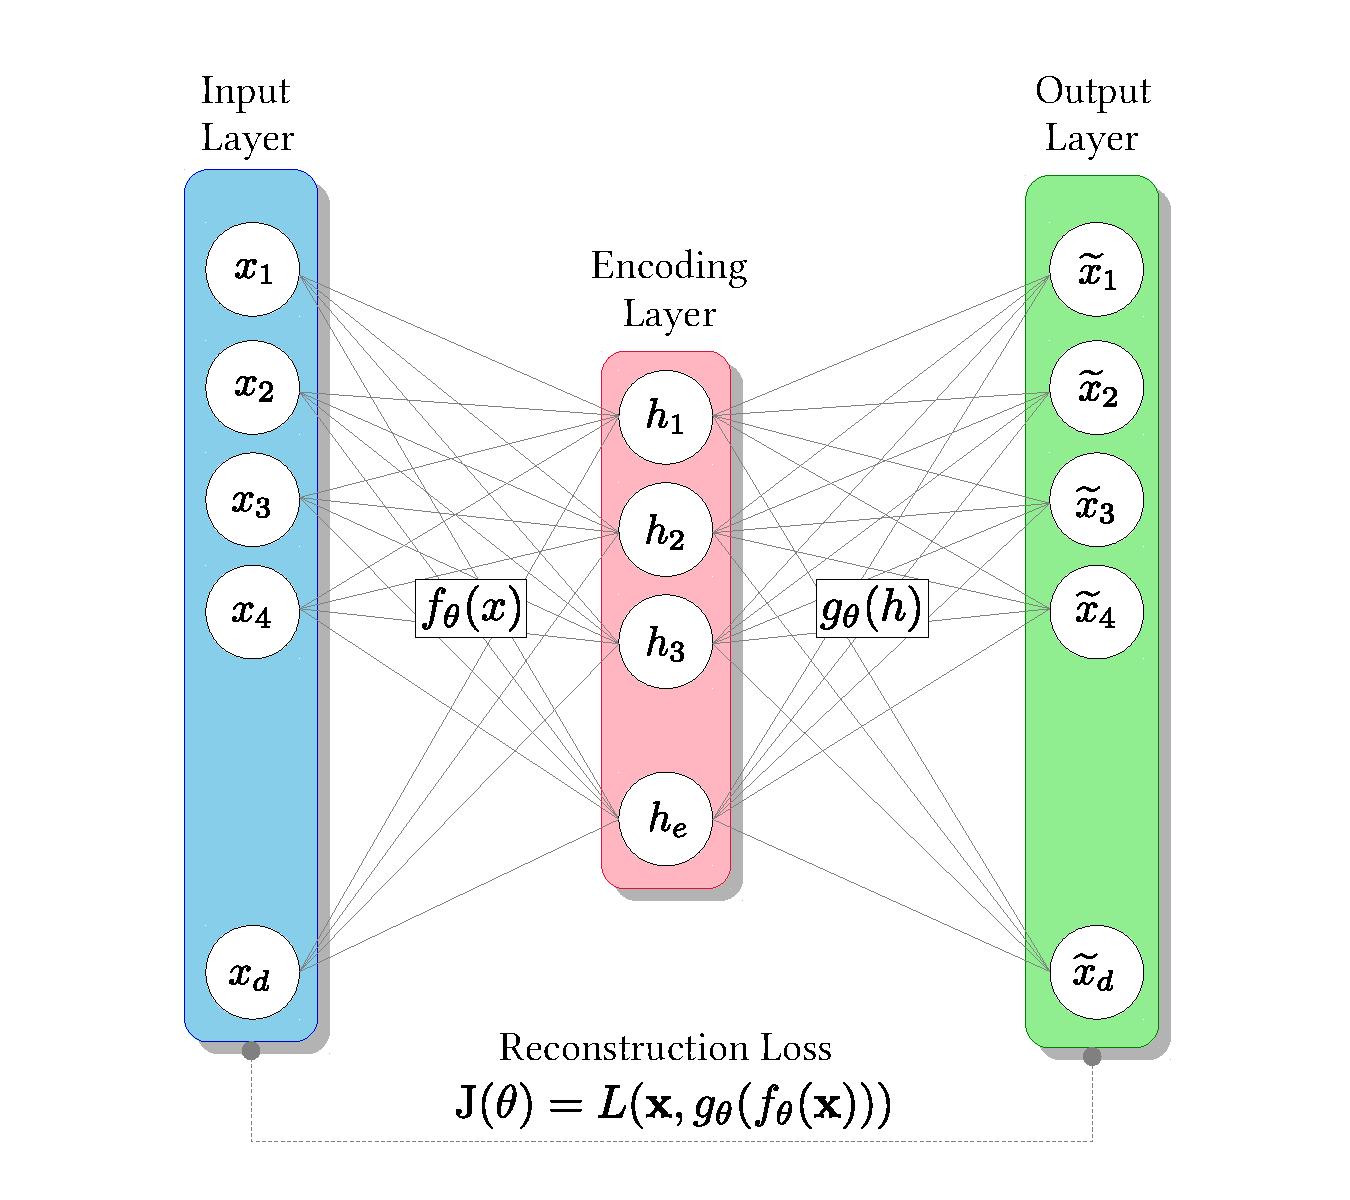
\includegraphics[width=0.40\textwidth]{ch01/schema_autoencoder}
  \caption[Diagram of the basic autoencoder]{
      Diagram of the basic autoencoder
  }
  \label{schema:autoencoder}
\end{wrapfigure}

\par This research is based on the autoencoder neural network as a framework
for solving the protein function prediction problem. It was first introduced
in 1987 (\cite{lecun1987phd}) and was subsequently studied in the following
years (\cite{bourlard1988auto, hinton1994autoencoders}). The idea is simple
yet powerful, that is, to have a network reconstruct a given input with the
presence of information bottlenecks.

\par There are two key aspects in training autoencoders: (1) information
reconstruction and (2) information bottleneck. The concept is that if an
autoencoder can reconstruct information ``perfectly'', even with constraints
involved, then it has learned the latent structure of the raw data. The
simplest way to constrain an autoencoder is by limiting the number of hidden
nodes $e$ less than the original dimension $d$ of the data. Say for example,
a dataset with $d=100$ dimensions. If we set $e=20$, and the autoencoder was
still able to reconstruct the original data ``perfectly'', then it has
learned a hidden structure from the data that was expressed in a lesser
capacity.

\par In practice, the autoencoder architecture consists of an encoder-decoder
scheme where the encoder function $f_{\theta}$ transforms the original input
$\mathbf{X}$ into a certain representation $\mathbf{h}$ (from $100$ features
to $20$), and the decoder function $g_{\theta^{\prime}}$ converts
$\mathbf{h}$ into an approximation of the raw features
$\mathbf{\widehat{X}}$ (where $\mathbf{\widehat{X}} =
g_{\theta^{\prime}}(\mathbf{h}) \approx \mathbf{X}$). Setting the loss
function as a comparison of the original input and its approximation
contrives the network to reconstruct $\mathbf{X}$:

\[
    J(\theta) = L(\mathbf{X}, \mathbf{\widehat{X}}) \quad \text{where} \quad
    \mathbf{\widehat{X}} = (g_{\theta^{\prime}} \circ f_{\theta}) (\mathbf{X})
\]

Algorithm \ref{algo:autoenc} describes the procedure for training an autoencoder.

%=============================================================================
% algo_autoenc.tex
% Copyright (c) 2018. Lester James V. Miranda
%
% This file is part of thesis-manuscript.
%
% thesis-mansucript is free software: you can redistribute it and/or modify
% it under the terms of the GNU General Public License as published by
% the Free Software Foundation, either version 3 of the License, or
% (at your option) any later version.
%
% thesis-manuscript is distributed in the hope that it will be useful,
% but WITHOUT ANY WARRANTY; without even the implied warranty of
% MERCHANTABILITY or FITNESS FOR A PARTICULAR PURPOSE.  See the
% GNU General Public License for more details.
%
% You should have received a copy of the GNU General Public License
% along with thesis-manuscript.  If not, see <http://www.gnu.org/licenses/>.
%
% Created by: Lester James V. Miranda <ljvmiranda@gmail.com>
%=============================================================================

\begin{algorithm}
    \caption{Training an autoencoder neural network}
    \label{algo:autoenc}
    \begin{algorithmic}[1]
    
    \INPUT Raw attributes $\mathbf{X}$
    \OUTPUT Learned parameters $\theta^{\ast}$

    \item[]
    \For{\textit{NumEpochs}}
        \State $\mathbf{h} \gets f_{\theta}(\mathbf{X}) = \sigma(\theta\mathbf{X}^{T} + \theta_0)$
        \Comment Encoder function
        \State $\mathbf{\widehat{X}} \gets g_{\theta^{\prime}}(\mathbf{h}) = \sigma(\theta^{\prime} \mathbf{h}^{T} + \theta^{\prime}_{0})$
        \Comment Decoder with tied-weights, $\theta^{\prime}=\theta^{T}$
        \State $J(\theta) \gets L(\mathbf{X}, \mathbf{\widehat{X}})$
        \Comment Compute loss
        \State \Call{Backpropagation}{$J(\theta)$}
        \Comment Optimize parameters
    \EndFor
    \State \Return $\theta^{\ast}$
    \Comment Return learned parameters
    \end{algorithmic}
\end{algorithm}

The learned parameters $\theta^{\ast}$ encapsulates the latent structure
discovered by the autoencoder. These parameters transform the original data
via the encoder function\textemdash i.e, $ \mathbf{X}^{\prime} =
f_{\theta^{\ast}}(\mathbf{X})$, $f_{\theta^{\ast}} \equiv \phi$\textemdash
and feed the transformation $\mathbf{X}^{\prime}$ into the multilabel
classifier $\mathcal{H}$. Figure \ref{schema:pipeline} illustrates this
simple model. In the next section, we will trace major developments in
protein function prediction via a machine learning approach that adheres
similarly to the figure above.

\begin{figure}[!t]
  \centering
  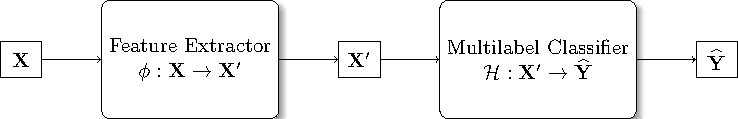
\includegraphics[width=0.85\textwidth]{ch01/schema_pipeline}
  \caption{Simple diagram of the protein function prediction model}
  \label{schema:pipeline}
\end{figure}

\section{Review of Related Literature}
\label{LiteratureReview}

\par There are three major movements one should consider when tracing the
developments in protein function prediction (PFP) in machine learning: first
is by (1) direct classification, then by (2) dimensionality reduction, and
lastly by (3) deep feature extraction. Machine learning techniques first
involved feeding raw data into a classifier, then found the need in reducing
the number of features in the dataset, and later on realized the importance
of learning suitable data representations for the classifier. This
research falls into the third category, utilizing deep neural networks to
learn representations for a multilabel classifier. But before that, let's
start from the beginning, where raw protein data is being fed directly to a
multilabel classifier.

\paragraph{Direct multilabel classification}
The earliest attempt to solve the protein function prediction problem was
done by \cite{elisseeff2001kernel}. They formulated PFP as a ranking problem
(not yet as a multilabel problem but rather an extension of multiclass
classification), and implemented a variant of the support-vector machine
(SVM) known as Rank-SVM. They tested their technique on \textit{S.
cerevisiae}, giving rise to the now known Yeast dataset. Later on,
\cite{diplaris2005protein} benchmarked various techniques on their own
protein data\textemdash the Genbase dataset. It is noteworthy that in the
conclusion of their work, they expressed their intention to investigate
``alternative representations of the learning problem,'' which brought a slew
of techniques for multilabel classification.

\par This brought forth the main baseline for multilabel classification, the
Binary Relevance (BR) algorithm
(\cite{godbole2004discriminative,tsoumakas2007multilabel}). These were then
extended into Label Powerset (LP) and Classifier Chains (CC)
(\cite{read2009classifier}), but BR's conceptual ease and ``relative speed''
enabled it to stay. Furthermore, various literature reviews attested BR's
performance, especially when paired with an SVM classifier
(\cite{luaces2012binary, zhang2014review,tsoumakas2017data}). For our
research, we will use the Binary Relevance with SVM (BR-SVM) as the baseline
of our work.

\paragraph{Reducing protein data dimensionality}
Although binary relevance has achieved good traction in protein function
prediction, training a classifier for each label can be time-consuming.
Researchers have then resorted to dimensionality-reduction techniques to
reduce the number of features in a protein\footnote{The Genbase dataset, for
instance, has $1186$ attributes} (\cite{wang2009using, wang2013protein,
wang2017protein}); they may not reduce the number of labels to train their
classifier upon, but they can perhaps reduce the time it takes to train one.
It is important to note that these techniques gave a semblance to feature
extraction. Reducing dimensions in a data may be akin to finding a different
representation of a feature space. However, dimensionality-reduction is still
limited primarily due to it being linear with less capacity
(\cite{cunningham2015linear}). In our work, we will compare against the work
of \cite{wang2013protein} that uses Principal Component Analysis (PCA) as a
dimensionality-reduction technique to a k-nearest neighbors classifier
(k-NN). They were able to reduce a protein dataset with $353$ features into
$204$, achieving good classification performance. We chose this method
because it follows a similar pipeline to Figure \ref{schema:pipeline}, and
uses a similar data source (gene expressions) to our protein benchmark.

\paragraph{Deep feature extraction in protein function prediction}
Reducing dimensions in protein data has sped-up and improved classification,
but common approaches such as principal component analysis (PCA) are linear
(\cite{bengio2013representation}), failing to capture the nonlinearities
present in a protein's feature space. This gave way for researchers to apply
deep learning techniques to protein data\textemdash both for protein
sequences (\cite{bhola2014machine,kulmanov2017deepgo, zou2017protein}) and
expressions (\cite{baldi2001bioinformatics, chicco2014deep}). Later on, we
will benchmark against \cite{chicco2014deep}, who used a deep autoencoder
network to extract features from protein gene expressions. Comparing against
this method enables us to have a baseline, traditional autoencoder
implementation to check our proposed architecture upon. As mentioned, this
research falls under the last category of deep feature extraction. This
method has been useful in aiding the classifier with a more separable feature
space, as demonstrated earlier by the XOR example. In addition, with Binary
Relevance, we can decouple the feature extractor from the multilabel
classifier to enable testing with different types of classifier.

\par However, we argue that extracting features is not enough. It is
important to learn representations relevant with respect to the classifier.
The next section elaborates this work's motivation\textemdash clarifying the
meaning of feature relevance\textemdash and formulate the problem and
research hypothesis throughout this work.

\section{Research Motivation}
\label{Motivation}

\par Learning new representations from raw protein data has been effective in
capturing nonlinearities in the feature space\textemdash a feat unachievable
by dimensionality reduction or direct classification. However, there is a
need to ensure that the extracted features are indeed \textit{relevant}. It
is important to have useful representations, not just linear combination of
features and weights optimizing a loss function. Given these, we state our
reseasrch motivation:

% State the motivation of this work: it's not enough to extract features
% it is also impmortant to extract relevant features.
\begin{quote}
  \itshape
  \small
  Although learning new representations from protein data has been explored
  in protein function prediction, we examine the effect of extracting
  relevant features to the predictive performance of a multilabel classifier.
  Hence, we propose two autoencoder-based techniques for motivating the
  extraction of such features. Our approach should improve a classifier's
  predictive performance, bringing us a step closer to a faster and more
  efficient annotation of protein functions.
\end{quote}

% enter relevance, define relevance, what does it mean to have a set of
% relevant features?
% use bengio and blum's definitions
\paragraph{Definitions of relevance}
\cite{blum1997selection} tackled the definition of relevance in their work.
According to them, feature relevance generally depends on the question:
``relevant to what?'' This means that features must be relevant
with respect to:
\begin{itemize}
  \item the target concept (i.e., \textit{labels}). \item the multilabel
  classifier (i.e., related to the task at hand)
\end{itemize}

\par They formulated various definitions of feature relevance depending on the
problem's goal. Because our main task is classification, we will adhere to
their definition of relevance as ``incremental usefulness'':

\begin{definition}
  \label{DefRelevance}
   Given a dataset $\mathcal{D}$, a learning algorithm $\mathcal{H}$ and a
   feature set $\mathbf{X}$. A feature set $\mathbf{X}^{\prime}$ is
   incrementally useful to $\mathcal{H}$ with respect to $\mathbf{X}$ if the
   accuracy of the hypothesis that $\mathcal{L}$ produces using
   $\mathbf{X}^{\prime}$\footnote{Adapted from \cite{blum1997selection}}
   is better than the accuracy achieved using just the
   feature set $\mathbf{X}$.
\end{definition}

\par\noindent For multilabel classification, we will be using a different set
of metrics instead of the accuracy. Originally, \cite{blum1997selection} uses
$\{x_{i}\} \cup \mathbf{X}$, but he goes at length extending this definition
to linear combinations of features, rather than just relevant individual
features\textemdash even citing PCA in the process. Simply put, this
validates the assumption that relevant features should produce better
predictions. In the next section, we will formulate the problem and state our
research hypothesis.

\subsection{Problem formulation}

\par The goal of this work is to extract a set of relevant features to
improve a classifier's performance in predicting protein functions. Formally,
the problem is defined as:

\begin{definition}
  Given a dataset $\mathcal{D}=\langle \mathbf{X}, \mathbf{Y} \rangle$ and a
  classifier $\mathcal{H}$, construct a feature extractor $\phi$ that learns
  a feature set $\mathbf{X}^{\prime}$ by $\phi: \mathbf{X} \rightarrow
  \mathbf{X}^{\prime}$ such that $\mathbf{X}^{\prime}$ is relevant with respect
  to $\mathcal{H}$ and $\mathbf{X}$ by virtue of Def. \ref{DefRelevance}.
\end{definition}

\par\noindent We will explore two different models that aim to accomplish
this task. Our research hypothesis is that by using the proposed feature
extractors $\phi^{\ast}$, relevant features $\mathbf{X}^{\prime}$ can be
produced and in consequence, improve the predictive performance of the
classifier $\mathcal{H}$.

\par The next chapter will discuss the Stacked Denoising Autoencoder (SdAE),
examining its denoising capability to obtain relevant features from an
inherently noisy protein dataset. SdAEs were originally used in image
denoising, yet this work will explore its efficacy in protein datasets in a
multilabel setting. The follow chapter will improve upon the autoencoder
architecture via a Mutually-Competitive autoencoder that learns a sparse and
relevant feature set by means of mutual competition. All of the resulting
features from these models will be fed into a BR-SVM classifier. We will test
this pipeline against the hypothesis that the features extracted using these
methods can improve the predictive performance of the classifier.
%=============================================================================
% Denoising Chapter
% Copyright (c) 2018. Lester James V. Miranda
%
% This file is part of thesis-manuscript.
%
% thesis-manuscript is free software: you can redistribute it and/or modify
% it under the terms of the GNU General Public License as published by
% the Free Software Foundation, either version 3 of the License, or
% (at your option) any later version.
%
% thesis-manuscript is distributed in the hope that it will be useful,
% but WITHOUT ANY WARRANTY; without even the implied warranty of
% MERCHANTABILITY or FITNESS FOR A PARTICULAR PURPOSE.  See the
% GNU General Public License for more details.
%
% You should have received a copy of the GNU General Public License
% along with thesis-manuscript.  If not, see <http://www.gnu.org/licenses/>.
%
% Created by: Lester James V. Miranda <ljvmiranda@gmail.com>
%=============================================================================

\chapter[Stacked Denoising Autoencoder for Protein Function Prediction]{
    \huge
    Feature Extraction using a Stacked Denoising Autoencoder for Protein
    Function Prediction
}
\label{SDAEChapter}

\par This chapter describes preliminary work where we extracted robust
features using a stacked denoising autoencoder (SdAE). Our main contribution
is that we have demonstrated the effectiveness of extracting features via
SdAE, commonly-used in images, in multilabel protein datasets. We start by
describing the SdAE architecture (Sec. \ref{SDArchitecture}), then illustrate
how it fits in the protein function prediction pipeline (Sec.
\ref{SDPipeline}). Then, we describe our experimental set-up (Sec.
\ref{SDSetup}), present results (Sec. \ref{SDResults}), and draw conclusions
(Sec. \ref{SDConclusions}).

\section{Stacked Denoising Autoencoder}
\label{SDArchitecture}

\begin{wrapfigure}{r}{0.53\textwidth}
  \centering
  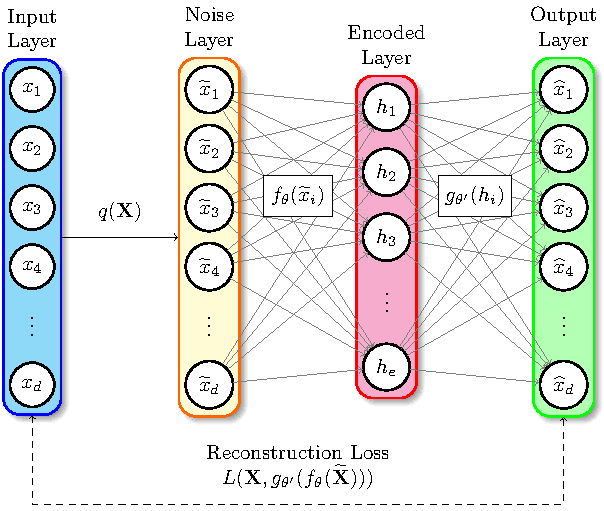
\includegraphics[width=0.5\textwidth]{ch03/sdae}
  \caption{Stacked denoising autoencoder}
  \label{schema:sdae}
\end{wrapfigure}

\par A stacked denoising autoencoder (SdAE) is a type of autoencoder that
corrupts the input data before reconstruction (\cite{vincent2010stacked}). It
is an extension of denoising autoencoders where layers are stacked and
greedily-trained\footnote{Greedy layer-wise training were once implemented
for practicality and to conserve memory (\cite{bengio2007greedy}). Today,
deep autoencoders like SdAE are trained end-to-end.}
(\cite{vincent2008denoising}).

\par Figure \ref{schema:sdae} illustrates the SdAE architecture. Given an
input data $\mathbf{X}$, we apply a corrupting function
$q(\mathcal{X}=\mathbf{X})$ to obtain a set of \textit{corrupted inputs}
$\mathbf{\widetilde{X}}$. We use the corrupted input to train the
autoencoder, but we compute the reconstruction loss by comparing the
reconstructed features $\mathbf{\widehat{X}}$ with the original data
$\mathbf{X}$. By learning from a set of corrupted inputs, we can capture the
``main factors of variations in the data (\cite{vincent2008denoising}),''
enabling our model to generalize unseen instances in the problem domain.
In theory, this should improve classification performance.

\subsection{More on generalization and manifold learning}

\begin{wrapfigure}{r}{0.5\textwidth}
  \centering
  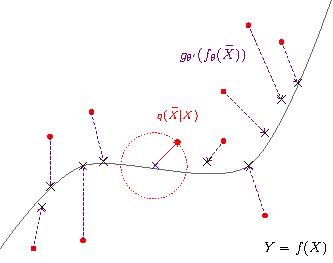
\includegraphics[width=0.45\textwidth]{ch03/demo_manifold}
  \caption[Manifold demonstration in SdAE]{Manifold learning in SdAE. Adapted
  from \cite{vincent2008denoising}}
  \label{demo:manifold}
\end{wrapfigure}

\par It is important to spend some time examining how corrupting inputs
during autoencoder training can enable generalization. Recall that
generalization prevents model overfitting, i.e. fitting too close to the
training set resulting to poor performance on the test set (represents unseen
or future data). Instead, what we want to do is obtain the main factors of
variation from the samples. Interpreting SdAEs this way permits us to apply
this method to a different domain\textemdash in this case, protein
data\textemdash with more confidence.

\par Say we're given a training dataset $X$ (marked by $\times$) that lies on
a manifold represented by the spline in Figure \ref{demo:manifold}. We don't
know what the spline looks like and the training data is not always
perfect.\footnote{The training data will not always be lying on-top of the
spline. We know this to be true because there will always be unmodeled
physics or measurement errors when obtaining the data that we cannot always
account, i.e., $x+\epsilon$} Our task is to learn the manifold which is
equivalent to identifying the structure of the spline. Applying the noise
function $q(\widetilde{X}|X)$ results to data points $\widetilde{x}$ (red
dots) that are further away from the spline. SdAE learns the manifold
(structure of the spline) by projecting these noisy inputs back to the spline
as demonstrated by the reconstructed inputs
$g_{\theta^{\prime}}(f_{\theta}(\widetilde{X}))$
(\cite{vincent2008denoising}). As we can see, the projections (purple lines)
can ``approximate'' the manifold and accommodate subtle variations even if a
new data point is slightly-off the spline. This idea is crucial given the
pretext that protein datasets are inherently noisy due to unaccounted
measurement errors (Sec. \ref{ProteinFunctionPrediction}).

\begin{figure}[h]
  \centering
  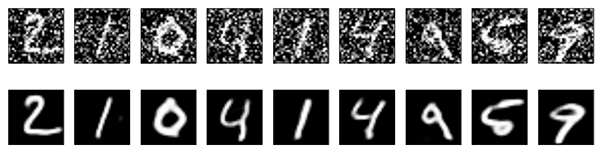
\includegraphics[width=0.9\textwidth]{ch03/demo_denoise}
  \caption[Demonstration of image denoising via SdAE]{
    Demonstration of image denoising via SdAE (\cite{chollet2016autoencoders})}
  \label{demo:denoise}
\end{figure}

\par Figure \ref{demo:denoise} provides a good demonstration of the
capabilities of SdAE in the MNIST dataset. It has learned to ``ignore'' the
unnecessary variations in the data (noise) while focusing on the structural
manifold of the image. As a result, it was able to reproduce cleaner images
from noisy samples. In context to our work, we can see that SdAE has learned
to distinguish between relevant and irrelevant aspects of the image: it
retained useful information (the actual digit) and discarded unnecessary ones
(random noise). 

\subsection{Practical considerations for SdAE training}

\par Table \ref{exp:noise_types} describes three different
corrupting functions for SdAE. We used the salt-and-pepper (SP)
noise because the dataset has been preprocessed by normalizing
the values in the range $(0,1)$. It is also a natural choice due
to the hidden representations being squashed by a sigmoid function.

\begin{table}[!h]
  \centering
  \caption[Different types of corrupting functions $q(\mathcal{X}) for SdAE$]
  {Different types of corrupting functions $q(\mathcal{X})$ for SdAE\\
  (\cite{vincent2010stacked})}
  \label{exp:noise_types}
  \begin{tabular}{@{}rp{0.70\textwidth}@{}}
      \toprule
      Noise                  & Description                                                   \\ \midrule
      Gaussian               & additive isotropic Gaussian noise $\mathbf{\widetilde{x}} |
                              \mathbf{x} \sim \mathcal{N}(\mathbf{x}, \sigma^2 I)$           \\
      Masking                & a random sample of elements in $\mathbf{x}$ are forced to $0$ \\
      Salt-and-Pepper        & a random sample of elements in $\mathbf{x}$ is set to their
                               maximum or minimum value (usually $0$ or $1$)                 \\\bottomrule
  \end{tabular}
\end{table}

\par We introduce a hyperparameter, noise rate ($r$), that dictates how much
of the elements in $\mathbf{x}$ will be affected by the noise. For
salt-and-pepper, this determines the percentage of features, that will be set
to $0$ or $1$ based on a coin flip (i.e., $P(0) = P(1) = 0.5$)


\par Lastly, Algorithm \ref{algo:sdae} describes the training procedure for SdAE.
It is similar to a deep autoencoder (Alg. \ref{algo:autoenc}), the only difference
is that we corrupt the inputs first. In the next section, we will present how
we incorporated SdAE in the protein function prediction pipeline.

%=============================================================================
% algo_sdae.tex
% Copyright (c) 2018. Lester James V. Miranda
%
% This file is part of thesis-manuscript.
%
% thesis-mansucript is free software: you can redistribute it and/or modify
% it under the terms of the GNU General Public License as published by
% the Free Software Foundation, either version 3 of the License, or
% (at your option) any later version.
%
% thesis-manuscript is distributed in the hope that it will be useful,
% but WITHOUT ANY WARRANTY; without even the implied warranty of
% MERCHANTABILITY or FITNESS FOR A PARTICULAR PURPOSE.  See the
% GNU General Public License for more details.
%
% You should have received a copy of the GNU General Public License
% along with thesis-manuscript.  If not, see <http://www.gnu.org/licenses/>.
%
% Created by: Lester James V. Miranda <ljvmiranda@gmail.com>
%=============================================================================

\begin{algorithm}
    \caption{Training a stacked denoising autoencoder}
    \label{algo:sdae}
    \begin{algorithmic}[1]
    
    \INPUT Raw attributes $\mathbf{X}$, Noise rate $r$
    \OUTPUT Learned parameters $\theta^{\ast}$

    \item[]
    \State $\mathbf{\widetilde{X}} \gets q(\mathbf{X}, r)$
    \Comment Corrupt inputs
    \For{\textit{NumEpochs}}
        \State $\mathbf{h} \gets f_{\theta}(\mathbf{\widetilde{X}}) = \sigma(\theta\mathbf{\widetilde{X}}^{T} + \theta_0)$
        \Comment Encoder function
        \State $\mathbf{\widehat{X}} \gets g_{\theta^{\prime}}(\mathbf{h}) = \sigma(\theta^{\prime} \mathbf{h}^{T} + \theta^{\prime}_{0})$
        \Comment Decoder with tied-weights, $\theta^{\prime}=\theta^{T}$
        \State $J(\theta) \gets L(\mathbf{X}, \mathbf{\widehat{X}})$
        \Comment Compute loss
        \State \Call{Backpropagation}{$J(\theta)$}
        \Comment Optimize parameters
    \EndFor
    \State \Return $\theta^{\ast}$
    \Comment Return learned parameters
    \end{algorithmic}
\end{algorithm}


\section{Protein Function Prediction Pipeline}
\label{SDPipeline}

\begin{figure}[!t]
  \centering
  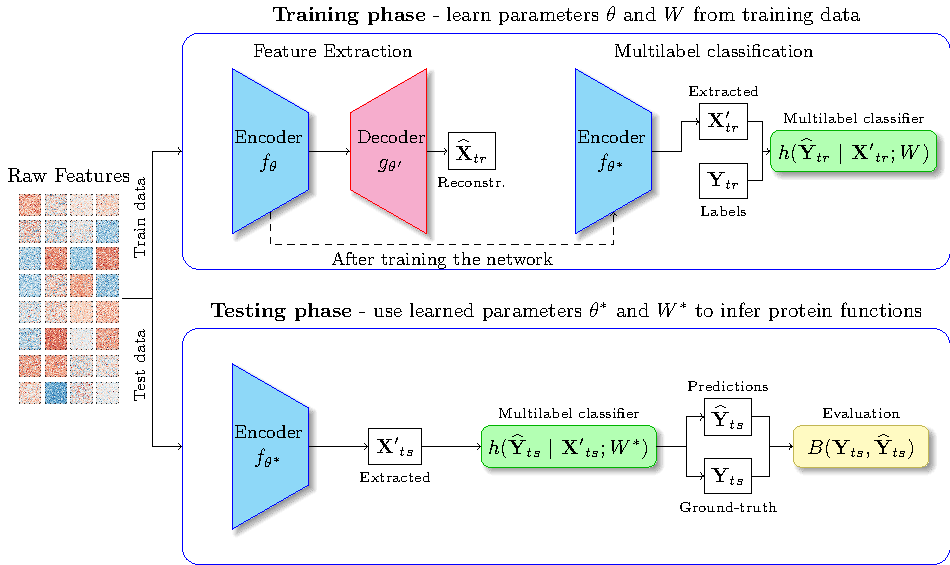
\includegraphics[width=0.90\textwidth]{ch03/schema_traintest}
  \caption[Protein function prediction pipeline]{Protein function prediction
  pipeline for the stacked denoising autoencoder}
  \label{schema:traintest_sdae}
\end{figure}

\par The protein function prediction pipeline consists of a (1) \textit{feature
extraction} and a (2) \textit{multi-label classification} stage as shown in
Figure \ref{schema:traintest_sdae}.\footnote{Except for the corruption part,
the pipeline in the mutually-competitive autoencoder (Chapter
\ref{SelectiveChapter}) looks exactly like this.} This follows the blueprint
introduced in Chapter \ref{Introduction} (Fig. \ref{schema:pipeline}); we
have a feature extractor $\phi$ that derives new features $X^{\prime}$, and
in turn, use them to train a multilabel classifier $\mathcal{H}$. Here, the SdAE
takes the role of the feature extractor, and a binary-relevance support-vector
machine (BR-SVM) as the classifier. Our main goal is to find the best set of
features $X^{\prime}$ that improves $\mathcal{H}$'s predictive performance.
As with standard machine learning practice, we have two phases\footnote{
  We usually split the dataset into training and test data such that
  $\mathcal{D} = \{\mathcal{D}_{tr}, \mathcal{D}_{ts}\}$. We didn't put the
  subscripts $tr$ and $ts$ for the features $\mathbf{X}$ and labels
  $\mathbf{Y}$ explicitly in all equations for it can be easily inferred
  which set is being used in which context.
}:

\begin{itemize}
  \item \textit{Training phase}: our goal is to learn the parameters $\theta$
  and $W$ for the extractor ($\phi$) and classifier ($\mathcal{H}$) stages
  respectively. We first train the SdAE using Alg. \ref{algo:sdae}, and use
  the learned $\theta^{\ast}$ to encode the training dataset for fitting
  BR-SVM. We use the mean-square error (MSE) as the loss-function for $\phi$ and
  L2-SVM for $\mathcal{H}$
  \begin{align}
    % Feature Extractor Loss
    \label{eqn:loss_fe_sdae}
    L(\mathbf{X},g_{\theta^{\prime}}(\mathbf{h}^{\prime})) &=
      \dfrac{1}{2}(\mathbf{X} - g_{\theta^{\prime}}(\mathbf{h}^{\prime}))^{2}\\
    % Multilabel classifier loss
    \label{eqn:loss_clf_sdae}
    J(\mathbf{X}^{\prime}, \widehat{\mathbf{Y}}, \mathbf{Y}) &= \sum_{\widehat{\mathbf{y}}_i \neq \mathbf{y}_{i}} \text{max}(0, W^{T}_{\widehat{\mathbf{y}}_{i}} \mathbf{x}_{i}^{\prime} - W^{T}_{\mathbf{y}_i}\mathbf{x}^{\prime}_i + \Delta)^2
  \end{align}
  \item \textit{Test phase}: this phase represents the scenario where we need
  to predict from unseen instances of protein data. We simply take the
  learned parameters $\{\theta^{\ast}, W^{\ast}\}$ and pass the test data
  through the encoder and classifier. The encoder derives new features given the
  equation: 
  \begin{align}
    % Encoder equation
    \label{eqn:encoder_mc_sdae}
    f_{\theta^{\ast}}(\mathbf{X}_{ts}) = \theta^{\ast T} \mathbf{X}_{ts} + \theta_{0}^{\ast}
  \end{align}
  
  \noindent for the classifier to infer upon. This produces a set of
  predictions $\mathbf{\widehat{Y}}_{ts}$ that we'll use to compare against a
  held-out set of ground-truth labels $\mathbf{Y}_{ts}$. We then evaluate
  these predictions using various metrics described in the next section.
\end{itemize}

\newpage
\subsection{Evaluation metrics}

To evaluate the performance of the prediction model, we will use the following
metrics\footnote[2]{\textit{tp}: true positive, \textit{fp}: false positive,
\textit{tn}: true negative, \textit{fn}: false negative}:

\begin{align}
    \text{Hamming Loss (H)} &= \dfrac{1}{N \cdot L} \sum_{i=1}^{N} \sum_{j=1}^{L}
    \text{XOR}(y_{ij}, \widehat{y}_{ij}) \\
    \text{Precision (P)} &=
    \dfrac{1}{N}\sum_{i=1}^{N}\dfrac{|\mathbf{\widehat{y}}_{i} \cap
    \mathbf{y}_{i}|}{|\mathbf{\widehat{y}_{i}}|} = \dfrac{tp}{tp + fp} \\
    \text{Recall (R)} &=
    \dfrac{1}{N}\sum_{i=1}^{N}\dfrac{|\mathbf{\widehat{y}}_{i} \cup
    \mathbf{y}_{i}|}{|\mathbf{\widehat{y}_{i}}|} = \dfrac{tp}{tp + fn} \\
    \text{F-score (F)} &=
    \dfrac{1}{N}\sum_{i=1}^{N} \dfrac{2 | \mathbf{\widehat{y}}_{i} \cup
        \mathbf{y}_{i}|}{|\mathbf{\widehat{y}}_{i} | + |\mathbf{y}_{i}|} =
        \dfrac{2 (\text{P} \cdot \text{R})}{\text{P} +
        \text{R}}
\end{align}

\par We will also compute for a fifth metric, the Area Under the ROC Curve
(AUROC), to serve as proxy for accuracy. For benchmarking, we will use the AUROC,
Hamming-Loss and F-score. Note that these metrics will exactly be the same for
our work on mutually-competitive autoencoders in Chapter \ref{SelectiveChapter}.

\section{Experimental Set-up}
\label{SDSetup}

\par We performed two (2) sets of experiments for the SdAE-based protein
function prediction pipeline. First, we checked how each hyperparameter,
i.e., noise rate ($r$) and number of encoding units ($e$) affects a
classifier's predictive performance. Then, we benchmarked our model against
different techniques in literature. Table \ref{exp:setup_sdae}
shows a summary of all experiments conducted in this work.

\begin{table}[h]
  \centering
  \caption{Summary of experiments}
  \label{exp:setup_sdae}
  \begin{threeparttable}
      \begin{tabular}{@{}rp{0.65\textwidth}@{}}
          \toprule
          Experiment & Description                                                            \\ \midrule
          \textit{Hyperparameter tests}                                                       \\
          Nb. of encoding units, $e$    & Test overcomplete and undercomplete configurations. \\
          Noise rate, $r$               & Sweep $k$-values in the range $\left[0,1\right]$    \\ \cmidrule{1-2} 
          \textit{Analysis \& benchmark}                                                      \\
          Model quality                 & Plot ROC and PR curves\tnote{1}                     \\
          Benchmark analysis            & Compare SdAE pipeline to other techniques\tnote{2}  \\ \bottomrule
      \end{tabular}
      \begin{tablenotes}
        \footnotesize
        \item[1] ROC - Receiver Operating Characteristic, PR - Precision--Recall
        \item[2] Friedman's test \parencite{friedman1937use} and post-hoc
        Bonferroni-Holm test \parencite{holm1979simple} were employed to
        measure statistical significance as recommended by
        \cite{demsar2006statistical}.
      \end{tablenotes}
    \end{threeparttable}
\end{table}

\par Lastly, Table \ref{exp:implementation_sdae} describes the implementation
environment for running the tests. The neural network was trained on an
NVIDIA Titan X (Pascal) GPU while the classifier was fitted using an Intel
Xeon 2.2GHz CPU. The majority of the code was written in Python 3.6.X using
the \href{https://www.tensorflow.org/}{Tensorflow} and
\href{https://keras.io/}{Keras} package. 

\begin{table}[t]
  \centering
  \caption{Experimental environment}
  \label{exp:implementation_sdae}
  \begin{threeparttable}
  \begin{tabular}{@{}rp{0.70\textwidth}@{}}
      \toprule
      Environment                    & Value                                             \\ \midrule
      \textit{Validation and testing}                                                    \\
      Number of trials               & 10: mean and std. dev. reported                   \\
      Train--validation--test split  & 50--30--20                                        \\ \cmidrule{1-2}
      \textit{Hardware dependencies}                                                     \\
      Number of cores\tnote{1}       & 10 in use (40 maximum)                            \\
      CPU                            & Intel Xeon 2.2GHz: Classifier training            \\
      GPU                            & NVIDIA Titan X (PASCAL): Neural network training  \\ \cmidrule{1-2} 
      \textit{Software dependencies}                                                     \\
      Language                & Python 2.7, 3.6 (compatible to both versions)            \\
      Libraries               & Tensorflow 1.2.1, Keras 2.1.2, Numpy 1.14.2              \\ \bottomrule
  \end{tabular}
  \begin{tablenotes}
    \footnotesize
    \item[1] We implemented a distributed scheme for training the classifier.
    Please see Appendix \ref{AppendixDistributed}.
  \end{tablenotes}
  \end{threeparttable}
\end{table}

\section{Results and Discussion}
\label{SDResults}

In this section, we'll present the results listed in Table
\ref{exp:setup_sdae}. First, we'll look into how different hyperparameter
settings\textemdash namely, noise rate ($r$) and number of encoding units
($e$)\textemdash affects the model as a whole. Then, we'll inspect the
quality of our model, and compare it with various works in literature.

\subsection{Characterizing the autoencoder model}

Our goal in this experiment is to find a pattern governing model behavior
with respect to different hyperparameter values. The idea is to take a
hyperparameter $\mathcal{P}$ and change its value while measuring the Area
under the ROC curve (AUROC). We then plot the results for both train and
validation data. We repeat this experiment for all datasets.

\subsubsection{Experiments on the Yeast Dataset}

Figure \ref{results:sdae_char_yeast} shows the characterization results for
Yeast. Recall that test set performance should always be lower than training
set performance, as the former simulates unseen samples. Here we can observe
the following:

\begin{itemize}
  \item Undercomplete autoencoders perform well without much overfitting.
  Overfitting can be observed with higher values of $e$, exemplified by the
  large gap between training and validation set performance; the model can
  predict the training data well, but fails to accommodate unseen instances
  of the validation data.
  \item Adding noise is beneficial, but too much noise can damage the model.
  Noise provides a good generalization ability to the model, and this
  confirms the ideas presented in denoising autoencoder literature (\cite{vincent2008denoising, vincent2010stacked}).
\end{itemize}
 
\begin{figure}[!t]
  \centering
  \begin{subfigure}[b]{0.48\textwidth}
    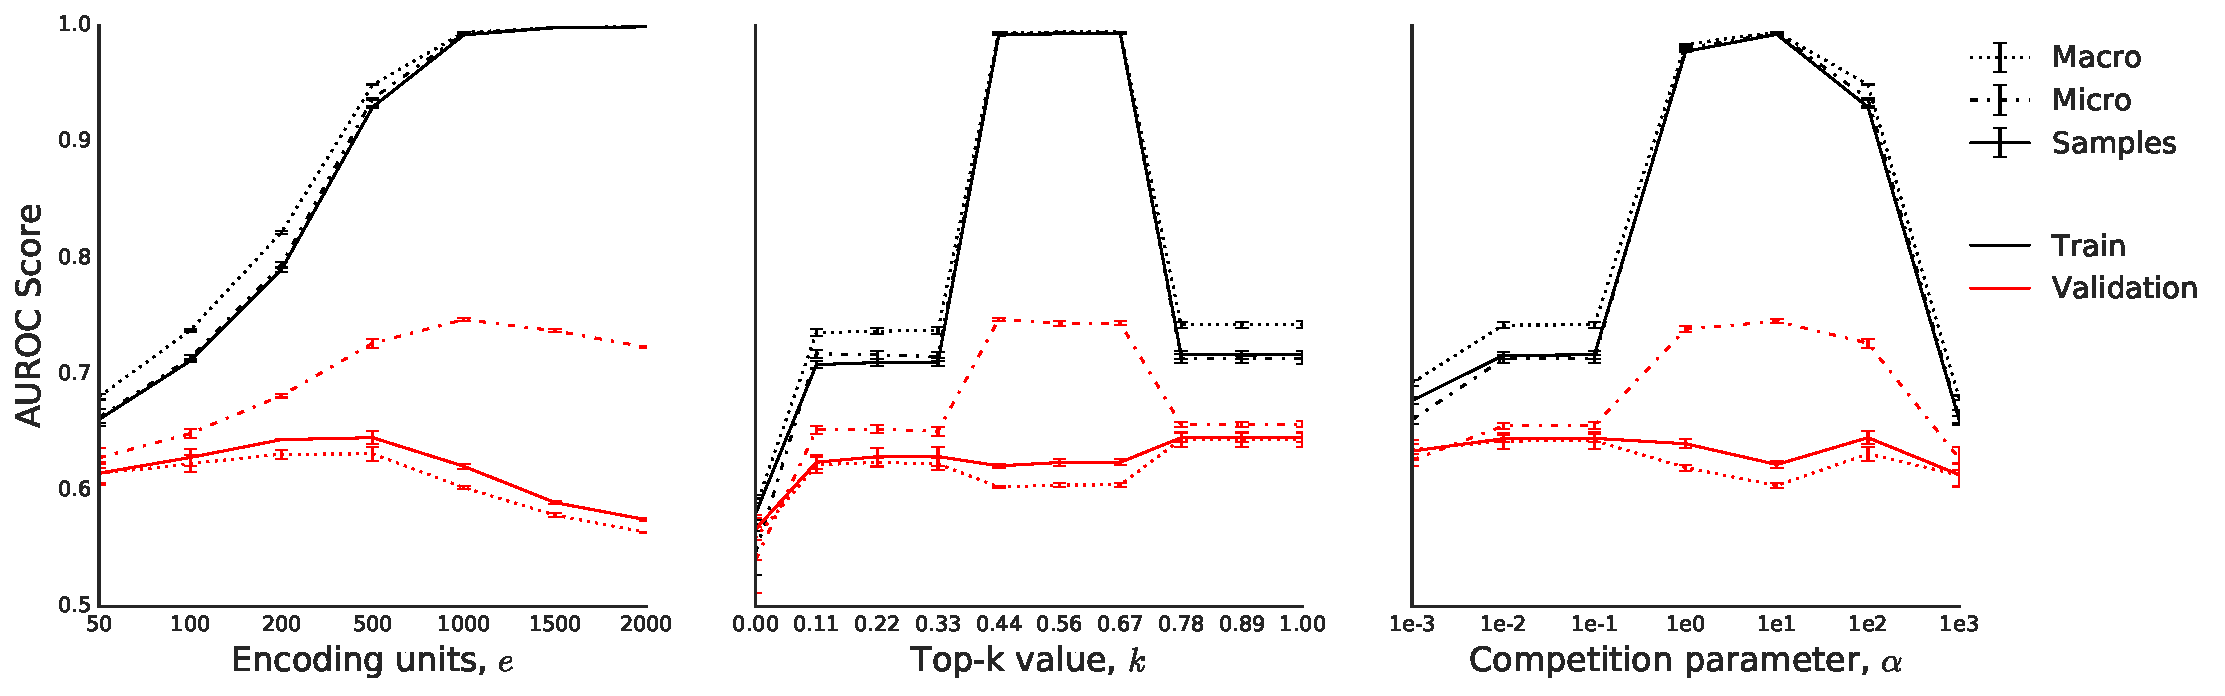
\includegraphics[width=\textwidth]{ch03/hyperparams_yeast}
    \caption{Yeast}
    \label{results:sdae_char_yeast}
  \end{subfigure}
  \begin{subfigure}[b]{0.48\textwidth}
    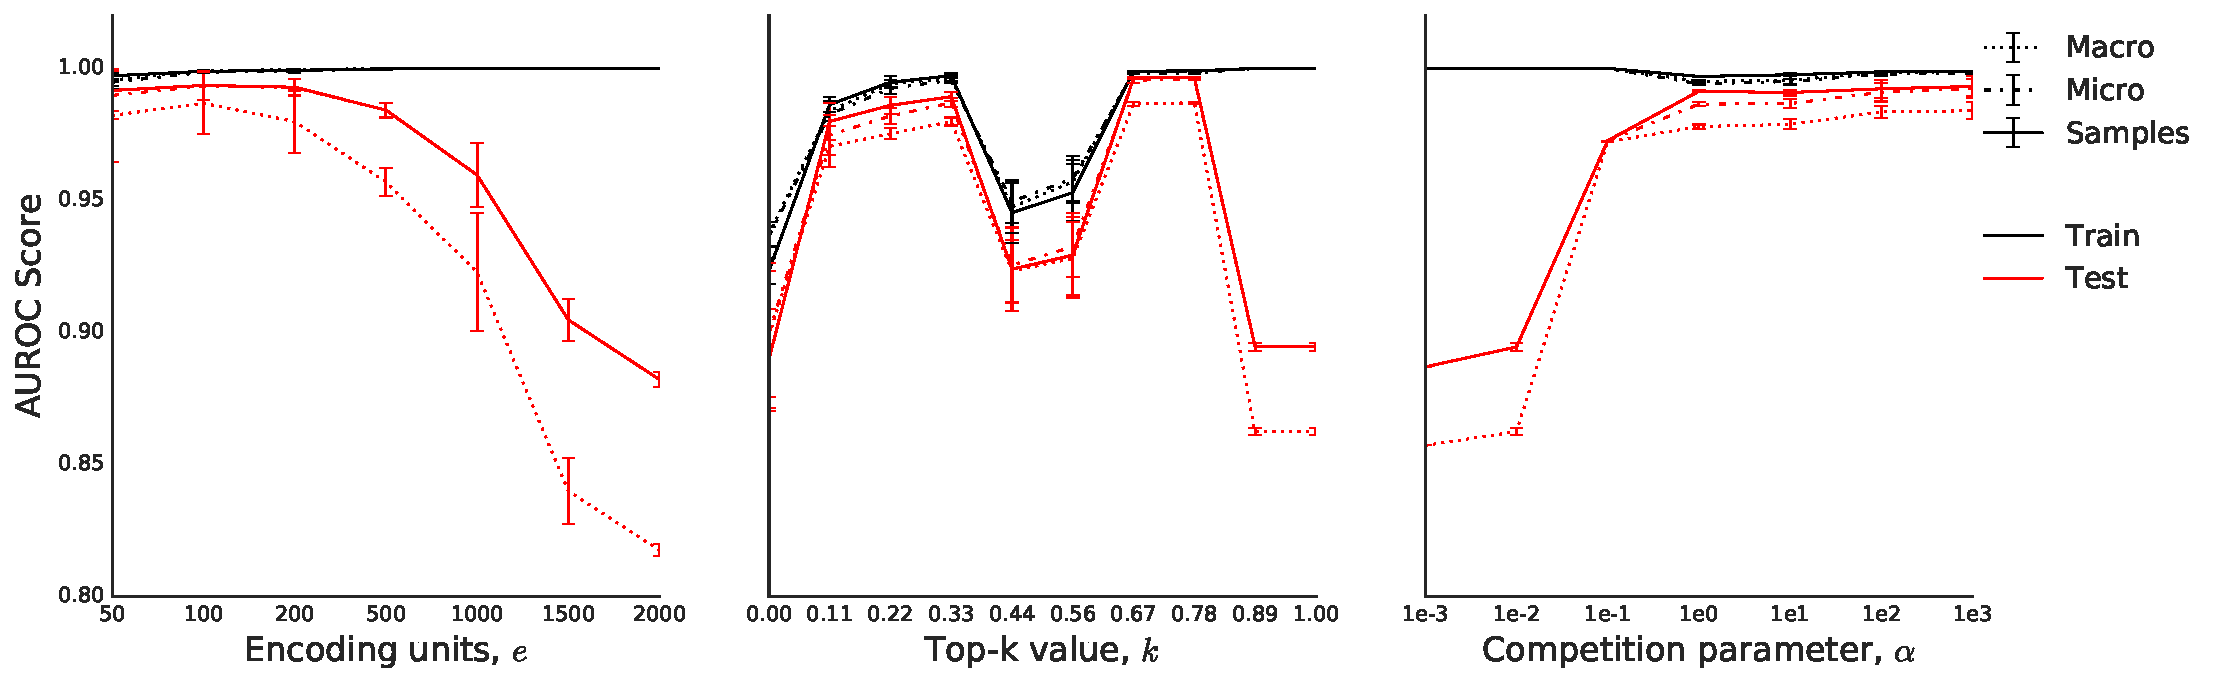
\includegraphics[width=\textwidth]{ch03/hyperparams_genbase}
    \caption{Genbase}
    \label{results:sdae_char_genbase}
  \end{subfigure}
  \caption{Model behavior on protein benchmarks}
  \label{results:sdae_char}
\end{figure}

\subsubsection{Experiments on the Genbase Dataset}

Figure \ref{results:sdae_char_genbase} shows the results for Genbase. A similar
procedure was performed for both training and validation data. We can infer
the following from the plots:

\begin{itemize}
  \item SdAE performance on Genbase is good overall. The small gap between
  training and validation performance shows that the model can perform well even
  with unseen instances of the data.
  \item Adding noise is also beneficial, but, similar to Yeast, may lead to
  overfitting if too much. Notice that validation performance is flat, this
  is due to the network having a smaller number of encoding units and shorter
  training time in this set-up ($e=50$ and $\text{epochs}=100$).
\end{itemize}

\subsection{Key results for the stacked denoising autoencoder}

In this section, we present our key results for the stacked denoising
autoencoder. First, we plot model quality in terms of the Receiver Operating
Characteristic (ROC) and Precision-Recall curves, then we present
benchmarking results against different models. Unlike the previous
experiment, we'll be reporting test set performance instead of the validation
set.

\subsubsection{Assessing model quality}

\par The goal of this experiment is to check if the proposed prediction
pipeline based on SdAE can indeed predict protein functions effectively. We
can achieve this by plotting the Receiver Operating Characteristic (ROC) and
Precision-Recall (PR) curves for both datasets and interpreting their shapes. 

\begin{figure}[!h]
  \centering
  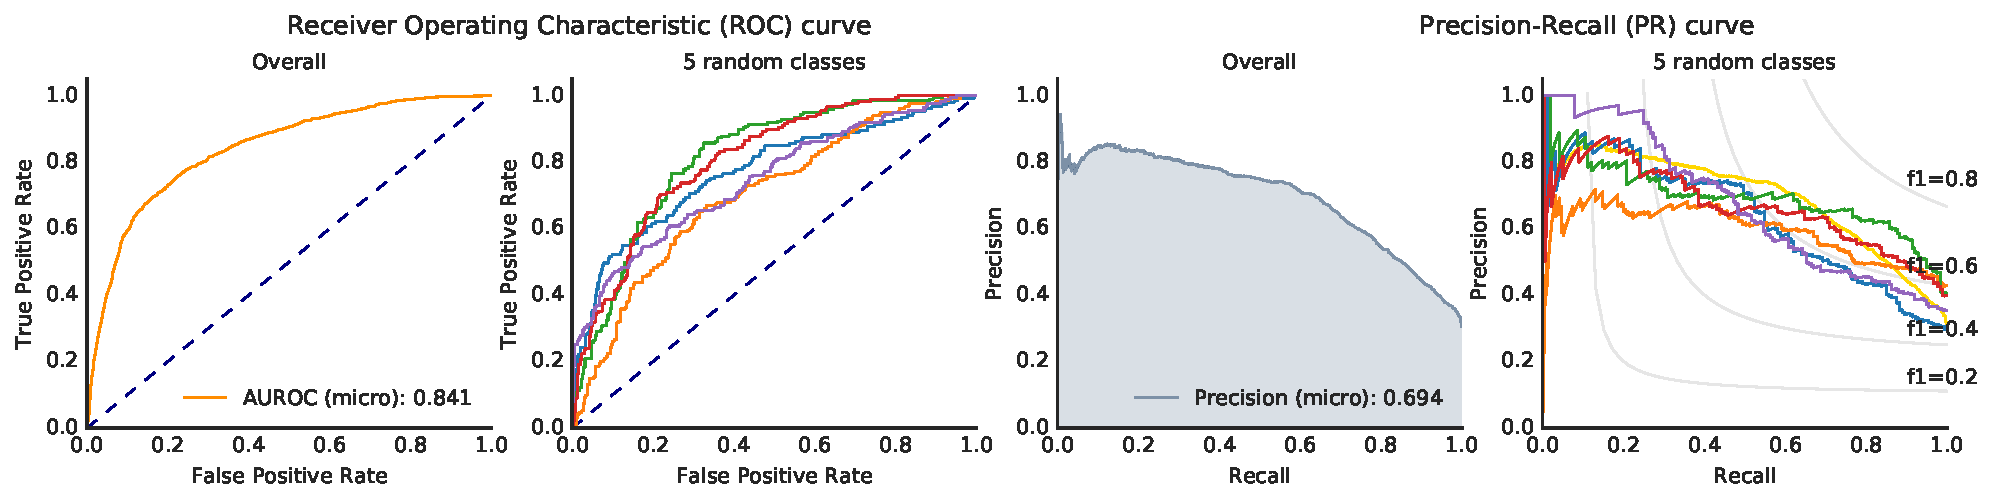
\includegraphics[width=0.95\textwidth]{ch03/ql_yeast}
  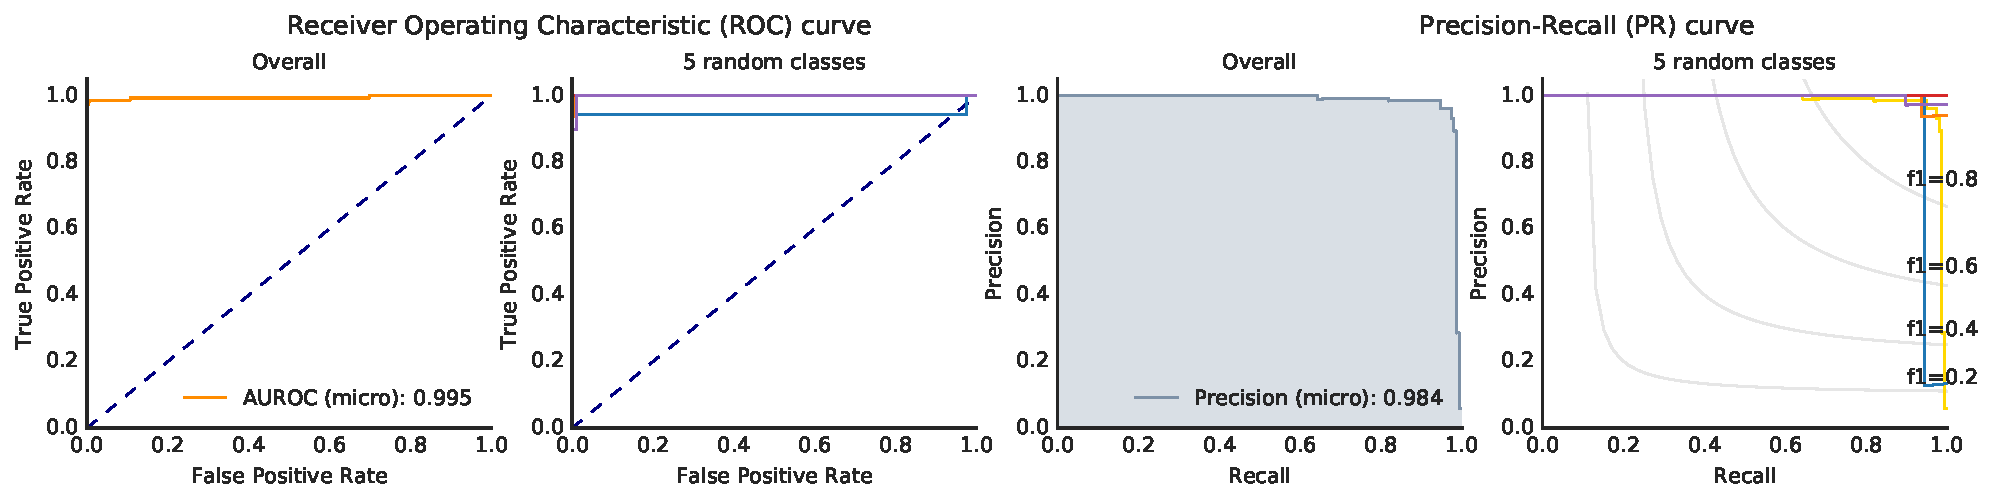
\includegraphics[width=0.95\textwidth]{ch03/ql_genbase}
  \caption[Receiver Operating Characteristic (ROC) and Precision-Recall (PR)
  curves for the two protein benchmarks]{
    Receiver Operating Characteristic (ROC) and Precision-Recall (PR) curves
    for both Yeast (\textit{top}) and Genbase (\textit{bottom}) datasets.
  }
  \label{results:sdae_quality}
\end{figure}


\par A good indicator of quality for an ROC curve is to check how far the
orange line, representing the FPR and TPR at different cutoff points, is from
the baseline (representing a random classifier). It is apparent that for both
datasets, the curve is way above the baseline\textemdash and moreso with
Genbase. In addition, measuring the AUROC gives a good predictive accuracy.
On the other hand, Precision-Recall curves show the tradeoff between
precision and recall for both datasets. It is apparent that Genbase has a
consistently high precision, whereas Yeast has decent quality. In the next
experiment, we'll put our prediction pipeline into context by comparing it
with other works in literature.


\subsection{Benchmark analysis}

\par In this experiment, we will compare against various protein function
prediction models in literature. The AUROC, F-score, and Hamming Loss will
measure model performance for both datasets. The results can be seen in
Tables \ref{results:sdae_benchmark_yeast} and
\ref{results:sdae_benchmark_genbase}

\par In addition, we conducted Friedman's test to assess significance in our
measurements. The null hypothesis $H_{0}$ dictates that there is no
significant difference between the groups. The ``Sig.'' column indicates the
extent in $\alpha$ in which we can reject $H_{0}$. The intuition is: the more
stars, the more confidence in the differences of the results.

\par For most metrics, the SdAE-based prediction pipeline performs well.
However, it is interesting that PCA (M1) and AE (M2) -based models have a
better AUROC performance. This can be attributed to some models having high
numbers of false negatives in their predictions, thus resulting to higher
accuracy given sparse labelsets. In fact, it may be easier to get high
accuracy by just predicting all samples as a zero-vector because of label
sparsity. However, if we look into the F-score metric, our model's
performance becomes more apparent. Our high F-score means that our prediction
pipeline can better ``balance'' between precision and recall (false positives
and false negatives). Lastly, an overall comparison using a post-hoc
Bonferroni-Holm test shows that our SdAE-based model outperforms other
models, especially the baseline. Outperforming the baseline is important
because it validates our claim that using feature extraction is beneficial to
multilabel classification.

\begin{table}[!t]
%
\centering
\begin{threeparttable}
\caption{Benchmark analysis on Yeast dataset}
\label{results:sdae_benchmark_yeast}
%
\begin{tabular}{@{}rr*{5}{l}@{}}
\toprule
        & & \multicolumn{5}{c}{Prediction Model\tnote{1}} \\ \cmidrule{3-6}
Metrics & Avg.      & Baseline       & M1             & M2                 & Proposed\tnote{2} & Sig.\tnote{3}\\
\midrule
AUROC   & micro     & \num{0.667(3)} & \num{0.666(2)} & \num{0.643(1)}     & \hg\num{0.668(4)}  & *** \\
        & macro     & \num{0.655(3)} & \num{0.659(2)} & \hg \num{0.662(1)} & \num{0.648(2)}     & *** \\
        & sample    & \hg\num{0.670(3)} & \num{0.656(2)} & \num{0.643(1)}  & \num{0.657(3)}     & *** \\
F-score & micro     & \num{0.548(4)} & \num{0.538(2)} & \num{0.530(1)}     & \hg\num{0.579(3)}  & *** \\
        & macro     & \num{0.597(4)} & \num{0.603(2)} & \num{0.590(1)}     & \hg\num{0.613(2)}  & *** \\
        & sample    & \num{0.536(3)} & \num{0.524(2)} & \num{0.517(1)}     & \hg\num{0.572(3)}  & *** \\
Hamming Loss & --   & \num{0.322(2)} & \num{0.343(2)} & \num{0.354(1)}     & \hg \num{0.231(3)} & *** \\
\bottomrule
\end{tabular}
%
\begin{tablenotes}
        \footnotesize
    \item[1] M1: \cite{wang2013protein}, M2: \cite{chicco2014deep}
    \item[2] Feature ext.: $\{r=0.75,e=103-100-80\}$, BR-SVM: $\{C=\num{1.00}, \gamma=\num{1.292e-2}\}$
    \item[3] Significance: *-$p\leq 0.1$, **-$p\leq 0.05$, ***-$p\leq 0.01$
\end{tablenotes}
%
\end{threeparttable}
%
\end{table}


\begin{table}[!t]
%
\centering
\begin{threeparttable}
\caption{Benchmark analysis on Genbase dataset}
\label{results:sdae_benchmark_genbase}
%
\begin{tabular}{@{}rrlllll@{}}
\toprule
        &        &  \multicolumn{5}{c}{Prediction Model\tnote{1}} \\ \cmidrule{3-6}
Metrics & Avg.   & Baseline       & M1             & M2             & Proposed\tnote{2}   & Sig.\tnote{3}\\
\midrule
AUROC   & micro  & \num{0.856(0)} & \hg\num{0.987(0)} & \num{0.974(10)} & \hg\num{0.987(1)}     & ***  \\
        & macro  & \num{0.671(0)} & \hg\num{0.992(0)} & \num{0.979(11)} & \num{0.983(1)}        & ***  \\
        & sample & \num{0.613(0)} & \num{0.950(0)}    & \num{0.976(10)} & \hg\num{0.988(1)}     & ***  \\
F-score & micro  & \num{0.671(0)} & \num{0.887(1)}    & \num{0.785(87)} & \hg\num{0.962(11)}    & ***  \\
        & macro  & \num{0.716(0)} & \num{0.950(0)}    & \num{0.892(40)} & \hg\num{0.964(6)}     & ***  \\
        & sample & \num{0.760(0)} & \num{0.928(0)}    & \num{0.810(95)} & \hg\num{0.970(8)}     & ***  \\
Hamming Loss & -- & \num{0.041(0)} & \num{0.014(2)}   & \num{0.035(17)} & \hg\num{0.005(1)}     & ***  \\
\bottomrule
\end{tabular}
%
\begin{tablenotes}
    \footnotesize
    \item[*] Values with $0.XXX(0)$ stdev. have deviations in the ten-thousandths place 
    \item[1] M1: \cite{wang2013protein}, M2: \cite{chicco2014deep}
    \item[2] Feature ext.: $\{r=0.60, e=1186-50\}$, BR-SVM: $\{C=\num{1.668e2}, \gamma=\num{2.154e-4}\}$
    \item[3] Significance: *-$p\leq 0.1$, **-$p\leq 0.05$, ***-$p\leq 0.01$
\end{tablenotes}
%
\end{threeparttable}
%
\end{table}


\begin{table}[!h]
%
\centering
\begin{threeparttable}
\caption{One-vs-All Overall Comparison\\using post-hoc Bonferroni-Holm Test\tnote{1}}
\label{results:sdae_stats}
%
\begin{tabular}{@{}r*{3}{l}@{}}
\toprule
Proposed Model vs.                       & Z-statistic    & $p$-value         & Sig.\tnote{2} \\ \midrule
Baseline                                 & $3.373282$      & $0.00057$         & ***          \\
\cite{wang2013protein}                   & $3.440050$      & $0.00116$         & **           \\
\cite{chicco2014deep}                    & $1.903010$      & $0.05704$         & ***          \\ \bottomrule
\end{tabular}
\begin{tablenotes}
\footnotesize
\item[1] Friedman's test rejects $H_{0}$ with $\chi^{2}=\num{9.37050}$.
\item[2] Significance: *-$p\leq0.1$, **-$p\leq0.05$, ***-$p\leq0.01$
\end{tablenotes}
\end{threeparttable}
\end{table}



\newpage
\section{Conclusion}
\label{SDConclusions}

\par We explored the effectiveness of a stacked denoising autoencoder (SdAE),
commonly-used in images, in the domain of protein function prediction. By
adding small perturbations in the input and using it to train a network, we
can produce a model with high generalization ability. We tested this process
on two protein benchmarks, and evaluated the predictions using various
metrics.

\par By characterizing the model's response given different hyperparameter
values, we found out that an autoencoder's configuration greatly affects the
overall model's predictive performance. For SdAE, an undercomplete hidden
layer is beneficial. Too high a number can cause model overfitting: high
performance in the training set but low performance during validation. In
terms of noise rates, it turns out that adding perturbations can indeed
improve classification performance. However, this value is entirely dependent
on the dataset, and must be probed using search techniques.

\par Then, we plotted ROC and PR curves to check if the resulting SdAE-based
model can indeed predict protein functions. We found out that the model is
fairly accurate and in fact, has a good balance between precision and recall.
We put these findings into context by comparing against other techniques in
literature. Results show that the SdAE-based model outperforms other
techniques in most metrics, especially the F-score. The accuracy for other
models is high, but this can be attributed to high false negatives given
sparse labelsets. The SdAE-based model's high F-score confirms this
hypothesis. Lastly, it is important to mention that using extracted features
outperforms a Baseline model without feature extraction. This validates our
hypothesis that extracting features is crucial in predicting protein
functions.

\par This work demonstrates that using a stacked denoising autoencoder can
aid in predicting protein functions. Furthermore, we have successfully
transferred SdAE into another domain, i.e., multilabel protein data. By
corrupting the inputs, the autoencoder is ``forced'' to sift through the data
and determine which inputs are relevant or not. However, we have no control
on how these relevant inputs are determined. Instead, we just let the network
greedily obtain new features and trust that the resulting features are
relevant. It is then important to add a degree of control in determining
relevant features, without risking information loss. In the next chapter, we
will introduce the mutually-competitive autoencoder, a neural network
architecture we designed to extract relevant features while preserving
information from the dataset.
%=============================================================================
% Mutual Competition Chapter
% Copyright (c) 2018. Lester James V. Miranda
%
% This file is part of thesis-manuscript.
%
% thesis-mansucript is free software: you can redistribute it and/or modify
% it under the terms of the GNU General Public License as published by
% the Free Software Foundation, either version 3 of the License, or
% (at your option) any later version.
%
% thesis-manuscript is distributed in the hope that it will be useful,
% but WITHOUT ANY WARRANTY; without even the implied warranty of
% MERCHANTABILITY or FITNESS FOR A PARTICULAR PURPOSE.  See the
% GNU General Public License for more details.
%
% You should have received a copy of the GNU General Public License
% along with thesis-manuscript.  If not, see <http://www.gnu.org/licenses/>.
%
% Created by: Lester James V. Miranda <ljvmiranda@gmail.com>
%=============================================================================

\chapter[Selective Feature Extraction via a Mutually-Competitive Autoencoder]{
    \huge
    Selective Feature Extraction using a Mutually-Competitive Autoencoder
    for Protein Function Prediction
} 
\label{SelectiveChapter}

%=============================================================================
% Conclusion
% Copyright (c) 2018. Lester James V. Miranda
%
% This file is part of thesis-manuscript.
%
% thesis-mansucript is free software: you can redistribute it and/or modify
% it under the terms of the GNU General Public License as published by
% the Free Software Foundation, either version 3 of the License, or
% (at your option) any later version.
%
% thesis-manuscript is distributed in the hope that it will be useful,
% but WITHOUT ANY WARRANTY; without even the implied warranty of
% MERCHANTABILITY or FITNESS FOR A PARTICULAR PURPOSE.  See the
% GNU General Public License for more details.
%
% You should have received a copy of the GNU General Public License
% along with thesis-manuscript.  If not, see <http://www.gnu.org/licenses/>.
%
% Created by: Lester James V. Miranda <ljvmiranda@gmail.com>
%=============================================================================
\chapter{Conclusion}
\label{ConclusionsChapter}

\par In this work, we have tackled the protein function prediction problem in
the angle of feature extraction: if we can extract \emph{better} features, then
we can obtain better predictions. Better features mean task-relevant and
meaningful representations of data, and by Def. \ref{DefRelevance}, can be
measured with an improvement in classification performance. 

\par Hence, we presented two autoencoder-based approaches geared towards the
extraction of relevant features: (1) a stacked denoising autoencoder-based
model that sifts through noise to obtain relevant features and (2) a
mutually-competitive autoencoder architecture that derives sparse yet relevant
representations. Our main hypothesis states that by using these methods, we can
generate relevant features, thereby inducing greater classification
performance. We tested our hypothesis on two protein benchmarks, Yeast and
Genbase, in a multilabel setting. There are two key insights in our work:


% Extracting relevant features is indeed crucial
\paragraph{Learning relevant features has benefit to classification.}
Features extracted from our two models have superior performance than other
techniques in literature. Specifically, we outperformed a
dimensionality-reduction approach (PCA) and a feature extractor not designed to
obtain relevant features (traditional autoencoder). More importantly, we
surpassed a baseline method without feature extraction. This shows that
although learning new representations is important, mere feature extraction is
not enough. It is crucial to ensure that the features we are deriving are
relevant to the task at hand. 

% Mutually-competitive autoencoder outperforms stacked denoising autoencoder
\paragraph{The mutually-competitive architecture outperforms the stacked
denoising autoencoder in most metrics} The architecture we designed in Chapter
\ref{SelectiveChapter} has greater performance than the stacked denoising
autoencoder (SdAE) in Chapter \ref{SDAEChapter} with respect to our problem
domain. We suggest two explanations for this behavior. First, the MC
autoencoder adds a higher degree of control during feature extraction. Aside
from the architecure, we can set three different hyperparameters to dictate the
flow of information in our network. Second, the autoencoder's strength lies on
its ability to prevent information loss while preserving data from the original
inputs. As we've seen in our ablation tests, the competition parameter that
reallocates neuron activations after winner-take-all has been beneficial to the
classifier's predictive performance. Thus, we not only learn the manifold, but
preserve more information to the relevant neurons.

\newpage
\par Next, we would like to list down the merits and major contributions of our
research:
\begin{itemize}
    \item In Chapter \ref{SDAEChapter}, we have successfully demonstrated the
        transferability of the stacked denoising autoencoder, commonly-used in
        images, to protein data within a multilabel setting. Learning the
        manifold via small perturbations in the input has been beneficial. More
        bottlenecks can lead to better generalization.
    \item In Chapter \ref{SelectiveChapter}, we have proposed an autoencoder
        architecture capable of extracting task-relevant representations of
        data. We have tested this on protein benchmarks and obtained good
        results. This architecture gives finer control during extraction, and
        performs even better than the denoising autoencoder approach.
    \item Overall, we have validated our claim that by extracting relevant
        features, we can improve the performance of a multilabel classifier in
        the protein domain. We obtained better performance when we're
        consciously extracting task-relevant features than by simple
        dimensionality-reduction or feature learning techniques.
\end{itemize}

\par In addition, it is also necessary to discuss some limitations in our work.
These can provide good jump-off points for further research:
\begin{itemize}
    \item \textit{It is difficult to interpret the extracted features from both
        models.} Although we know that these features help the classifier, it
        is difficult to distinguish what they truly represent (cell binding
        sites, sequence length, etc.). By nature, neural network models are
        black-boxes, and if we're optimizing for accuracy, we might sacrifice
        interpretability.
    \item \textit{Our work does not cover hierarchical labels.} There may be
        cases where labels also have a relationship with one another: a
        ``husky'' is a ``dog'' as ``cellular bud site selection'' is a
        ``mitotic cell cycle process.'' Our protein benchmarks all have flat
        labels, and thus these cases were not considered. 
\end{itemize}

\par Lastly, here are some suggestions for future work:
\begin{itemize}
    \item \textit{Better model interpretability for autoencoder networks.} This
        is a huge area of research and may involve the use of generative
        methods such as variational autoencoders.
    \item \textit{Improve handling of data imbalance.} There are cases when one
        label is more dominant to the other, affecting classification
        performance. A more balanced dataset can boost classifier performance.
    \item \textit{Consider label information during autoencoder training.} This
        is relevant when hierarchical labels are involved. Our feature
        extractor is unsupervised, and it may be interesting to see a
        supervised approach to autoencoder training.
\end{itemize}

\par Applying machine learning to the problem of protein function prediction is
a herculean task. It requires careful thought not only in classifying
multilabel data, but also of how proteins are represented to the classifier.
We have shown that by procuring task-relevant protein representations, we can
aid the classification of protein functions. We hope that through our methods,
we can add value to this fundamental task, and pave way to the development of
advanced medicine and better healthcare for the society. $\blacksquare$



%------------------------------------------------------------------------------
%	THESIS CONTENT - APPENDICES
%------------------------------------------------------------------------------

\appendix % Cue to tell LaTeX that the following "chapters" are Appendices

% Include the appendices of the thesis as separate files from the Appendices folder
% Uncomment the lines as you write the Appendices

% \include{Appendices/AppendixA}
%\include{Appendices/AppendixB}
%\include{Appendices/AppendixC}

%------------------------------------------------------------------------------
%	BIBLIOGRAPHY
%------------------------------------------------------------------------------

\printbibliography[heading=bibintoc]

%------------------------------------------------------------------------------

\end{document}  
